%------------------------------------------------------------
%	CAPITULO I
%------------------------------------------------------------

\chapter{Desarrollo de la skill}
\label{capIV}

El Buscador Gavilán, es una skill basada en reconocimiento de voz que tiene como objetivo mejorar el proceso de investigación y búsqueda de información por medio de una metodología formal de búsqueda, llamada Modelo Gavilán, detallado en el capítulo \ref{capII} del presente trabajo.

Por otra parte, el diseño de la skill toma bases teóricas del diseño de interfaces de usuario, ajustadas para las interfaces basadas en voz, tal como guías y principios mencionados en el capítulo \ref{capIII}. Algunas guías sobresalientes utilizadas son las siguientes:

\begin{itemize}
  \item Navegación en la interfaz
  \item Facilidad de entrada de datos
  \item Manipulación directa
  \item Lenguaje natural
\end{itemize}

También se consideran algunos principios de las ocho reglas de oro del diseño de interfaces, mostradas a continuación:

\begin{itemize}
  \item Usabilidad universal
  \item Comentarios o respuestas informativas
  \item Diálogos para término de acciones
  \item Prevención de errores
  \item Fácil retroceso de acciones
  \item Reducción de carga de memoria a corto plazo
\end{itemize}

Para el desarrollo del diseño de la skill, se toma como base una metodología basada en el diseño centrado en el usuario, la cual consiste en diseñar un sistema orientado a satisfacer las necesidades de los usuarios que harán uso de un producto o servicio. El diseño centrado en el usuario considera un proceso dividido en cuatro partes.

\begin{itemize}
  \item \textbf{Especificar el contexto de uso.} Para conocer de forma más cercana a los usuarios, se realizó una investigación del proceso de búsqueda de información con alumnos de licenciatura, con el fin de conocer la forma en que habitualmente realizan una investigación.
  \item \textbf{Especificar los requisitos.} Con el fin de identificar las necesidades del usuario, se desarrollaron herramientas para conocer la forma en las que se pueden satisfacer. En esta etapa se desarrollaron dos modelos para la técnica Persona, uno para un alumno de preparatoria y otro para un alumno de licenciatura, en los que se plantean sus intereses, objetivos, experiencias, entre otros.
  \item \textbf{Producir soluciones de diseño.} Con la información anterior, se presentó una serie de posibles soluciones por medio de un Customer Journey Map, en el que se realizaron ajustes e identificaron puntos de provecho para la implementación de la skill. Por otra parte, se crearon algunas propuestas para el diseño de la navegación por el sistema, en la que se agregaron mejoras hasta llegar a una versión estable para la implementación.  
  \item \textbf{Evaluación.} Con el fin de evaluar de forma precisa la usabilidad del sistema, se contó con cinco usuarios, con los cuales se aplicaron las pruebas basadas en el proceso de evaluación del grupo ESIE.
\end{itemize}

Dados los resultados obtenidos de todo el proceso de diseño, se logró una versión estable para su implementación, cuyo código se encuentra en un servicio de Amazon para el diseño de skills llamado Alexa Developer Console.

%------------------------------------------------------------
%	Alexa Amazon
%------------------------------------------------------------

\section{Alexa Amazon}
\label{AlexacapIV}

% REFERENCIA
Amazon (2022a), señala que Alexa es el servicio de voz de la compañía Amazon, disponible para los dispositivos de Amazon, tales como Amazon Echo, Echo Dot, Echo Pop y Echo Show, así como dispositivos terciarios con Alexa integrada. Por medio del servicio de Alexa, se crean capacidades y habilidades más personalizadas para los usuarios, llamadas skills. Alexa es un servicio que funciona por el reconocimiento por voz, de tal forma que cuando un usuario emite algún sonido o comando por voz, Alexa procesa la entrada y da una respuesta acorde a la información solicitada.

% REFERENCIA
Amazon (2022b) señala que el servicio Alexa Voice Service (AVS) provee todas las herramientas para poder integrar de forma correcta el servicio de reconocimiento por voz de Amazon. La documentación del servicio AVS provee los documentos para el desarrollo e identificación de requerimientos del producto, así como guías especializadas para desarrolladores.

Cabe recalcar que existe una gran diferencia entre los servicios de Alexa y Alexa Voice Service. Alexa es un servicio que se encarga de dar mantenimiento y función a los dispositivos Amazon Echo, mientras que AVS es un servicio enfocado a fabricantes de dispositivos comerciales. Entre estos fabricantes, se encuentran aquellos que utilizan AVS para incorporar Alexa en diferentes tipos de dispositivos, tales como altavoces, auriculares, computadoras, televisores, vehículos, entre otros dispositivos categorizados como inteligentes.

% REFERENCIA
AVS es un servicio que se puede apoyar de algunas herramientas que provee el equipo de desarrollo de Amazon (2022b), tales como las siguientes:

\begin{itemize}
  \item Alexa Built-in Product (ABI). Es una categoría de dispositivos que tienen integrado AVS, así como micrófonos, altavoces y un conjunto de funciones de Alexa para activación de palabras.
  \item AVS Device SDK. Son bibliotecas hechas en el lenguaje de programación C++, que utiliza las APIs de AVS. Estas bibliotecas facilitan y agilizan la integración de las características y funcionalidades de Alexa.
  \item APIs de Alexa. Son APIs para la implementación y automatización para directivas en la nube y eventos de un cliente.
\end{itemize}

% REFERENCIA
Alexa (2022b) recomienda considerar la respuesta de una serie de preguntas para el mejor diseño y desarrollo de un producto que utilice AVS. Entre estas preguntas se encuentran las siguientes:

\begin{enumerate}
  \item ¿Dónde será usado el producto por los clientes?
  \item ¿Este dispositivo agrega Alexa a espacios como el hogar, la oficina, habitaciones, vehículos o estará a dondequiera que vaya el cliente?
  \item ¿Que tipo de fuente de alimentación necesitará?
  \item ¿Accede a la nube de AVS por medio de Wifi o dependerá de Bluetooth y una aplicación móvil?
  \item ¿Cómo interactúa con los clientes?
  \item ¿Puede hablar con el dispositivo directamente o es necesario emparejarlo con otros dispositivos integrados a Alexa?
  \item ¿A qué distancia deben estar del dispositivo?
  \item ¿Cómo iniciarán la interacción?
  \item ¿Tendrá pantalla?
  \item ¿Qué pueden hacer los clientes con el producto?
\end{enumerate}

Es importante considerar estas características, ya que permiten tener una visión general del funcionamiento y casos de uso del producto o dispositivo final. La última pregunta del listado anterior, enfoca su contenido a la consideración de la incorporación de las funcionalidades con las que cuenta Alexa, tales como las que se muestran a continuación:

\begin{itemize}
  \item Activar a Alexa con la voz o el tacto, así como interrumpirla con la voz y el tacto.
  \item Permitir que transmita y controle música.
  \item Permitir la transmisión de sonido grupal en varias habitaciones de forma síncrona.
  \item Crear, detener y cancelar temporizaciones, alarmas y recordatorios.
  \item Recibir y eliminar notificaciones.
  \item Ver el contenido como tarjetas de visualización para dispositivos con pantalla.
  \item Emparejar dispositivos a través de Bluetooth.
  \item Mantener el contacto con llamadas, mensajes o anuncios.
  \item Presionar algún botón para hablar con Alexa, controlar el audio o alternar micrófonos.
\end{itemize}

%------------------------------------------------------------
%	Skills
%------------------------------------------------------------

\subsection{Skills}
\label{SkillscapIV}

% REFERENCIA
Alexa cuenta con diferentes funcionalidades, en las que se encuentran las skills. Amazon (2022c) define una skill como funcionalidades que permiten a los consumidores crear una experiencia más personalizada para realizar diferentes tareas. En pocas palabras, las skills son aplicaciones desarrolladas para el servicio de Alexa.

Las skills necesitan una palabra o comando para poder activarse. Un usuario puede activar una skill utilizando alguna palabra de activación, tal como $"$comienza$"$, $"$abre$"$ o $"$inicia$"$, seguido del nombre de la skill que se desea activar. Gracias al reconocimiento por voz y el procesamiento del lenguaje natural incorporado en Alexa, se reconoce el comando para que la skill solicitada se ejecute como un servicio en una plataforma en la nube. La forma de comunicación entre una petición y la nube se basa en el protocolo HTTPS, siendo la solicitud un verbo de tipo POST que contiene un payload de tipo JSON con el contenido necesario para dar respuesta al usuario por medio de Alexa.

En la Figura \ref{fig:41} se muestra el flujo de procesamiento para invocar una skill con Alexa.

\begin{figure}[H]
% \begin{figure}
  \centering
  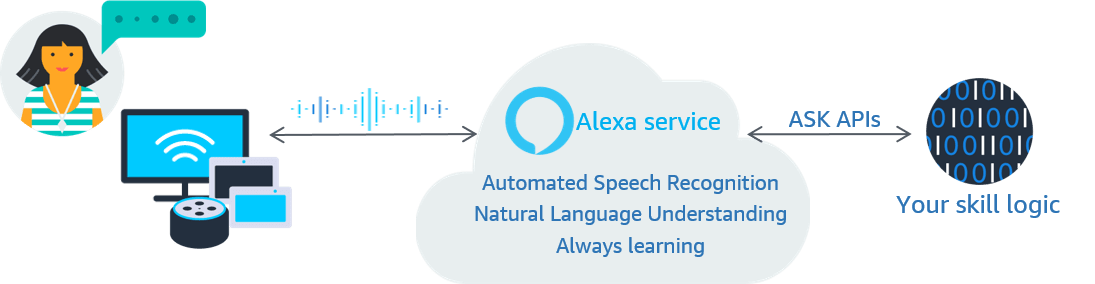
\includegraphics[width=0.70\textwidth]{Cap4/Figuras/ProcesoInvocacionSkill.png}
  \caption{Flujo de procesamiento de activación por voz para invocar una skill. Amazon (2022d).}
  \label{fig:41}
\end{figure}

%------------------------------------------------------------
%	Alexa Skills Kit (ASK)
%------------------------------------------------------------

\subsubsection{Alexa Skills Kit (ASK)}
\label{ASKcapIV}

% REFERENCIA
Amazon (2022c) señala que las skills se apoyan de un conjunto de herramientas para poder ser desarrolladas, llamado Skills Kit (ASK), que es el conjunto de herramientas, documentación, APIs, guías y ejemplos, que permiten el desarrollo y mantenimiento de las skills para Alexa de una forma sencilla y rápida.

Entre las herramientas que ofrece el ASK, se encuentran las siguientes:

\begin{itemize}
  \item La consola de desarrollo de Alexa, la cual contiene distintas opciones para respaldar el ciclo de vida de desarrollo.
  \item Bibliotecas que dan acceso a las funcionalidades de Alexa.
  \item Herramientas para poner a prueba la skill, tal como el simulador de funcionalidades de Alexa.
  \item Solucionador de problemas de reconocimiento de voz y procesamiento de lenguaje natural.
  \item Proporciona apartados para certificar y publicar la skill.
  \item Herramientas para administrar y monitorear las skills.
  \item Guía de diseño de Alexa para realizar las mejores prácticas de diseño de skills y modelos de interacción de voz personalizadas.
  \item Proporciona una biblioteca de intents para las expresiones más comunes.
  \item Documentación técnica, tutoriales y ejemplos de código para apoyar el proceso de creación de una skill.
\end{itemize}

%------------------------------------------------------------
%	Modelos de interacción de las skills
%------------------------------------------------------------

\subsubsection{Modelos de interacción de las skills}
\label{ModelosInteraccioncapIV}

% REFERENCIA
Amazon (2022e), señala que cada skill cuenta con un modelo de interacción de voz, en cual define las frases y palabras que un usuario puede decir mientras una skill está activada. De tal forma que cuando un usuario hace alguna solicitud, Alexa, con ayuda del ASK, toma como base el modelo de interacción de la skill para interpretar la solicitud y realizar la acción específica.

Alexa permite definir dos tipos de modelos de interacción de voz para las skills. Estos modelos se mencionan a continuación:

\begin{itemize}
  \item \textbf{Modelo de interacción de voz preconstruido.} El ASK determina el conjunto de palabras o frases que los usuarios dicen para invocar una skill. Las invocaciones de este modelo están enfocadas a solicitudes ya predefinidas.
  \item \textbf{Modelo de interacción de voz personalizado.} En este modelo el desarrollador diseña toda la interacción de voz, en la que se definen todas las formas en las que un usuario se puede comunicar y cómo la skill responde a cada tipo de solicitud definida en el modelo.
\end{itemize}

% REFERENCIAS
Para los dos tipos de modelo de interacción de voz, se debe definir el modelo sobre el que se va a basar la skill. Amazon (2022e) menciona algunos pasos recomendables para diseñar el modelo de interacción de una skill:

\begin{enumerate}
  \item Definir los intents que la skill puede reconocer. Los intents son acciones que un usuario puede realizar dentro de una skill. Se hablará a detalle más adelante.
  \item Definir los utterances, que son los enunciados o frases que los usuarios pueden decir para invocar un intent. Como un usuario puede solicitar una acción de diferentes formas, existe un mapeo de muchos enunciados a un intent.
  \item Definir el nombre que usará Alexa para identificar la skill. Este es el nombre con el que el usuario podrá formar el comando de activación de la skill.
  \item Opcionalmente, se pueden definir elementos visuales e interacciones táctiles para dispositivos que cuentan con una pantalla táctil con integración de Alexa.
  \item Definir la lógica de la skill para cumplir las intenciones personalizadas.
\end{enumerate}

Es importante recalcar que cualquier tipo de modelo de interacción por voz usa el mismo mecanismo de comunicación descrito en la Figura \ref{fig:41}.

%------------------------------------------------------------
%	Tipos de Skill
%------------------------------------------------------------

\subsubsection{Tipos de Skill}
\label{TiposSkillcapIV}

% REFERENCIA
Las skills que pueden ser desarrolladas tienen una clasificación definida por el ASK. Amazon (2022f) propone una clasificación que define el tipo de la skill según su modelo de interacción de voz, sus capacidades y características.

La Tabla \ref{tab:t41} describe los distintos tipos de skills, así como su enfoque.

\begin{table}[H]
  \begin{center}
    \begin{tabular}{ | p{4cm} | p{4cm} | p{8cm} | }
      \hline
      TIPO DE LA SKILL & MODELO DE VOZ & DESCRIPCIÓN  \\ \hline
      Automotive & Preconstruido y personalizado & Skills adaptadas a un automóvil. \\ \hline
      Business & Preconstruido & Skills que brindan acceso de voz a reuniones, calendarios comerciales, reserva de salas, etc. Este tipo también incluye skills enfocados a la hotelería y residencia. \\ \hline
      Cooking & Preconstruido & Skills para controlar y conectarse con aparatos de cocina. \\ \hline
      Custom & Personalizado & Skills con un modelo de interacción personalizado para la interacción con el usuario. \\ \hline
      Entertainment Device & Preconstruido & Skills que permiten controlar dispositivos inteligentes como televisores, altavoces, entre otros. \\ \hline
      Flash Briefing & Preconstruido & Skills que proporcionan información como noticias o contenido breve de Flash Briefing. \\ \hline
      Games & Personalizado & Skills enfocadas a la interacción con juegos manejados por voz. Estas skills se apoyan fuertemente de imágenes para dispositivos con pantalla. \\ \hline
      Knowledge & Knowledge & Skills que permite a los usuarios conocer información sobre cálculos de una organización sin invocar el nombre de la skill. \\ \hline
      List & Personalizado & Skills que permiten leer y actualizar las listas de un usuario de Alexa. \\ \hline
      Music, Radio, and Podcast & Preconstruido & Skills que permiten controlar audio transmitido a través de los dispositivos habilitados para Alexa. \\ \hline
      Networking and Wi-Fi & Preconstruido & Skills para modelar redes Wi-Fi domésticas. \\ \hline
      Smart Home & Preconstruido & Skills que permiten controlar los dispositivos domésticos inteligentes. \\ \hline
      Smart Home Energy & Preconstruido & Skills que permiten administrar el uso de energía de Alexa. \\ \hline
      Smart Home Security & Preconstruido & Skills que permiten controlar dispositivos de seguridad domésticos inteligentes, tales como cámaras, cerraduras, sensores de movimiento, entre otros. \\ \hline
      Video & Preconstruido & Skills que permiten controlar dispositivos de video, así como consumir video. \\ \hline
    \end{tabular}
    \caption{Tipos de Skill según su enfoque}
    \label{tab:t41}
  \end{center}
\end{table}

%------------------------------------------------------------
%	Flujo de desarrollo de una Skill
%------------------------------------------------------------

\subsubsection{Flujo de desarrollo de una Skill}
\label{FlujoSkillcapIV}

% REFERENCIA
Amazon (2022d) señala que el desarrollo de cualquier tipo de skill sigue un proceso de diseño, creación e implementación que se divide en cinco etapas.

\begin{enumerate}
  \item \textbf{Diseñar la skill.} Consiste en diseñar un modelo de interacción por voz de tal forma que la conversación sea natural y se base en un diseño centrado en el usuario. 
  \item \textbf{Construir la skill.} Esta etapa consiste en implementar el modelo de interacción de voz. Para los modelos de interacción personalizados, la skill se construye a partir de las herramientas que provee ASK y un entorno de desarrollo apropiado para el lenguaje de programación seleccionado para su implementación.
  \item \textbf{Probar la skill.} Las pruebas de la skill pueden hacerse fácilmente sin un dispositivo, utilizando el simulador de Alexa, que se encuentra incorporado en la consola de desarrollo de Alexa. En este simulador se pueden definir varias características, tales como los diferentes dispositivos y la interacción multimodal.
  \item \textbf{Certificar y publicar la skill.} Antes de que una skill sea publicada en la tienda de Skills de Alexa, se debe pasar por un proceso de certificación para asegurar que cumpla todos los requisitos de calidad, seguridad y políticas de Amazon. Si todas las pautas se cumplen, la skill estará disponible en la tienda de skills de Amazon para los usuarios de Alexa. 
  \item \textbf{Supervisar la skill.} Es posible monitorear el uso de la skill en vivo, así como ejecutar un análisis y consultar las ganancias en caso de haber. 
\end{enumerate}

Este proceso se sigue como en la Figura \ref{fig:42}.

\begin{figure}[H]
% \begin{figure}
  \centering
  \includegraphics[width=0.70\textwidth]{Cap4/Figuras/Flujo de creación de skill.jpg}
  \caption{Flujo de creación de una skill. Amazon (2022d).}
  \label{fig:42}
\end{figure}

%------------------------------------------------------------
%	Alexa Developer Console
%------------------------------------------------------------

\subsection{Alexa Developer Console}
\label{ADCcapIV}

La consola de desarrollo de Alexa es una herramienta que se encuentra contenida en el ASK. Su objetivo es brindar un control del flujo de creación de una skill.

La consola de desarrollo de Skills se divide en cinco secciones:

\begin{itemize}
  \item \textbf{Skills.} Listado de las skills desarrolladas en la cuenta de Amazon.
  \item \textbf{Ganancias.} Se muestran datos informativos sobre las ganancias generadas con las skills publicadas en la tienda de skills de Amazon.
  \item \textbf{Pagos.} Se muestra información de los pagos realizados durante un periodo.
  \item \textbf{Alojamiento.} En este apartado se presenta información relacionada al uso de algunos servicios de Amazon Web Services (AWS), tales como AWS Lambda, Amazon S3, Amazon DynamoDB, entre otros.
  \item \textbf{Configuraciones.} Se muestra información de administración del acceso a la skill, gestión de usuarios e id's.
\end{itemize}

Estas opciones se encuentran en la presentación de la consola de desarrollo de Alexa, tal como se muestra en la Figura \ref{fig:43}.

\begin{figure}[H]
% \begin{figure}
  \centering
  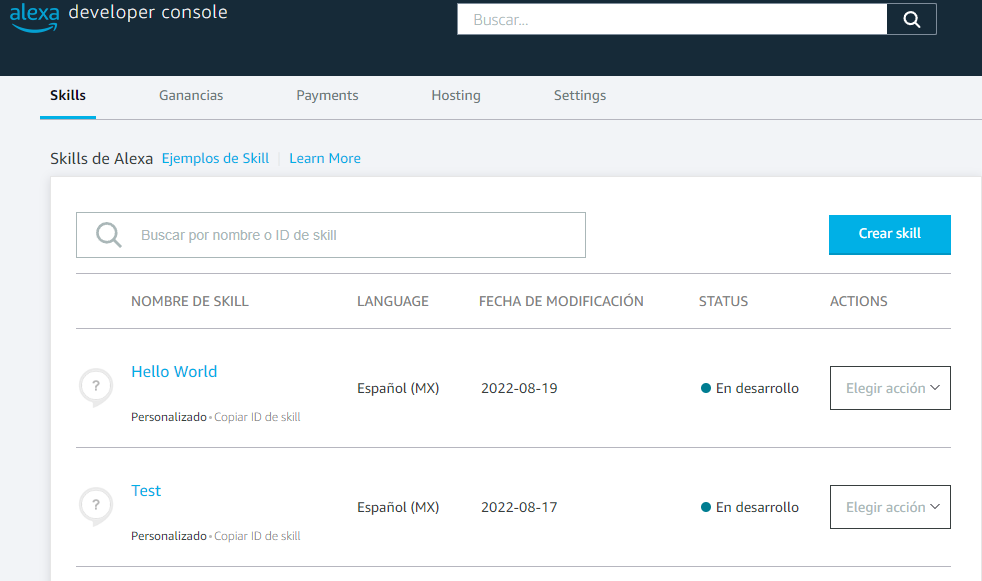
\includegraphics[width=0.60\textwidth]{Cap4/Figuras/Consola de Desarrollo de Alexa.png}
  \caption{División de la consola de desarrollo de Alexa.}
  \label{fig:43}
\end{figure}

La consola de desarrollo de Amazon también provee el flujo de creación de una skill por cada proyecto en desarrollo, en espera de certificación o publicado. El flujo definido se muestra a continuación:

\begin{enumerate}
  \item \textbf{Construcción (Build).} En esta sección se crean y configuran los siguientes elementos.
  \begin{itemize}
    \item Invocación o invocaciones.
    \item Intenciones.
    \item Declaraciones.
    \item Slots.
  \end{itemize}
  \item \textbf{Código (Code).} Apartado en el que se encuentra todo el código del comportamiento y funcionamiento de la skill. En este apartado se declara la función lambda, que es la función principal donde se programa el funcionamiento de la skill.
  \item \textbf{Pruebas (Test).} Contiene el simulador de Alexa, en el cual se pueden realizar pruebas sobre el funcionamiento de la skill.
  \item \textbf{Distribución (Distribution).} Información requerida para publicar la skill, tales como el nombre, descripción, logo, entre otros. En este apartado se define la siguiente información:
  \begin{itemize}
    \item Nombre público de la skill.
    \item Descripción breve de la skill.
    \item Descripción detallada de la skill.
    \item Funcionalidades generales de la skill.
    \item Frases de ejemplo para invocar la skill y manejar el flujo durante su ejecución.
    \item El ícono de la skill.
    \item La categoría de la skill.
    \item Palabras clave de la skill.
    \item URL de políticas de privacidad de la skill.
    \item URL de términos y usos de la skill.
    \item Determinar si la skill permite a los usuarios realizar pagos o gastar dinero real.
    \item Determinar si la skill permite acciones de compra a los usuarios.
    \item Determinar si la skill recopila información personal de los usuarios.
    \item Determinar si la skill está dirigida a usuarios menores a trece años.
    \item Determinar si la skill contiene publicidad.
    \item Aceptar los términos de cumplimiento de exportación de la skill.
    \item Instrucciones para realizar pruebas sobre la skill antes de ser publicada.
    \item Determinar si la skill es pública o su acceso está restringido a organizaciones de negocios.
    \item Decidir si se habilita la distribución automatizada de configuraciones regionales.
    \item Seleccionar la región en la que estará disponible la skill dentro de la tienda de skills.
  \end{itemize}
  \item \textbf{Certificación (Certification).} Sistema de validación de requerimientos y reglas para publicar la skill. En este apartado se presentan las siguientes acciones:
  \begin{itemize}
    \item Verificar que la skill no infringe políticas declaradas por Amazon.
    \item Información sobre las veces que se ha validado la skill y sus resultados.
    \item Historial de versiones de la skill.
    \item Un comparador para relacionar dos variantes de una misma skill y encontrar sus diferencias.
  \end{itemize}
  \item \textbf{Analítica (Analytics).} Información sobre la administración y analíticas del uso de la skill. Se puede encontrar la siguiente información:
  \begin{itemize}
    \item Un resumen del uso del modelo personalizado de la skill.
    \item La cantidad de veces que la skill se ha activado.
    \item Métricas del uso de sesiones, intenciones, declaraciones, entre otros.
    \item Información sobre el performance de la skill.
  \end{itemize}
\end{enumerate}

Estos apartados se encuentran organizados en pestañas dentro de la configuración de una skill, tal como se muestra en la Figura \ref{fig:44}.

\begin{figure}[H]
% \begin{figure}
  \centering
  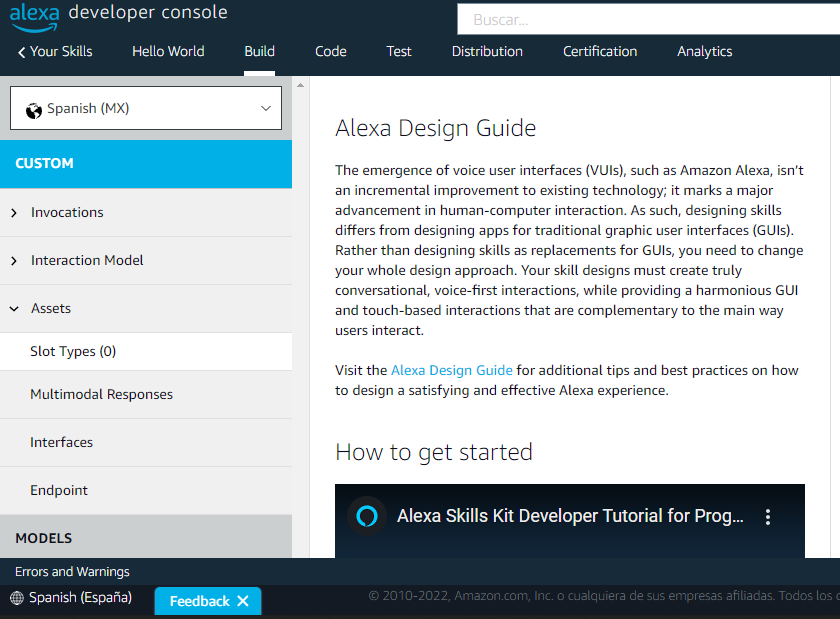
\includegraphics[width=0.60\textwidth]{Cap4/Figuras/Proceso de creacion de skill.png}
  \caption{Flujo del proceso de creación de skills.}
  \label{fig:44}
\end{figure}

%------------------------------------------------------------
%	Invocaciones
%------------------------------------------------------------

\subsubsection{Invocaciones}
\label{InvocacionescapIV}

% REFERENCIA
Amazon (2022g) una invocación como las diferentes formas en las que se puede activar una skill para comenzar a ejecutarse en el servicio de Alexa. La invocación de una skill puede ser ajustada y editada durante el proceso de desarrollo, sin embargo, la invocación no puede cambiar una vez que la skill ha sido certificada y publicada, por lo que es importante definir una invocación adecuada desde la etapa de diseño y configuración.

Las invocaciones se encuentran dentro de la sección llamada Build, tal como se muestra en la Figura \ref{fig:45}.

\begin{figure}[H]
% \begin{figure}
  \centering
  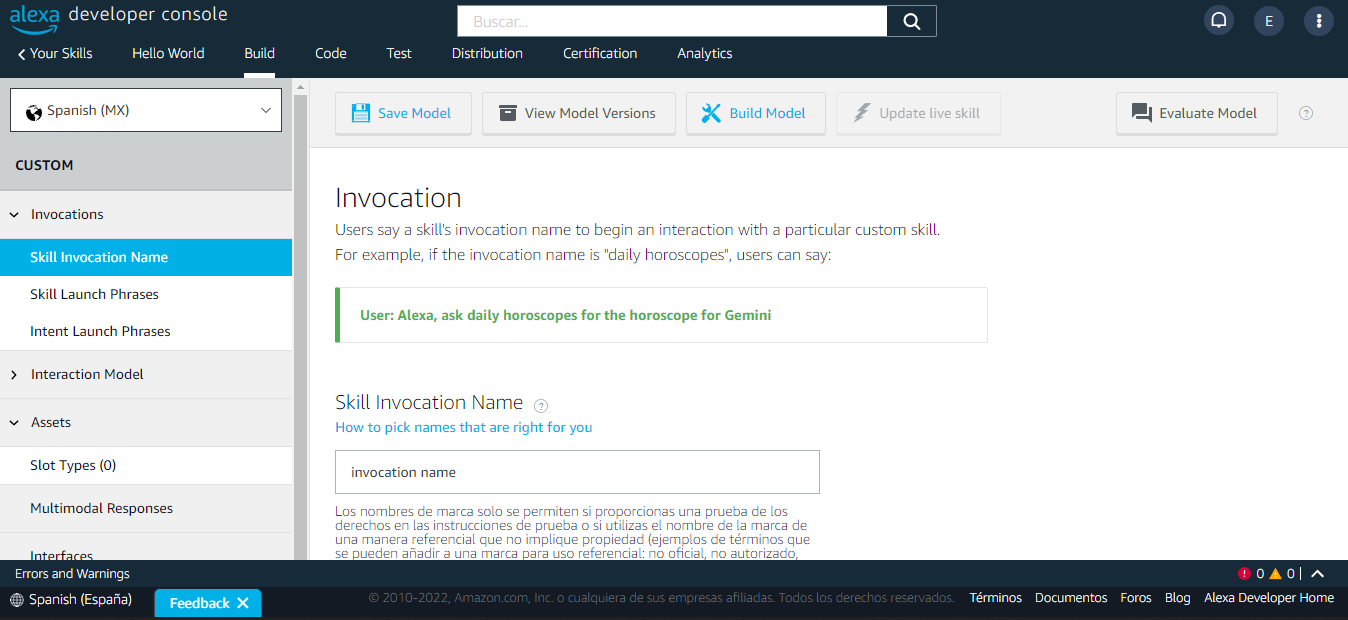
\includegraphics[width=0.70\textwidth]{Cap4/Figuras/Invocaciones.png}
  \caption{Definición de invocación o invocaciones de una skill.}
  \label{fig:45}
\end{figure}

Las invocaciones son un concepto que es aplicable únicamente para las skills personalizadas, ya que las skills pre-construidas requieren definirlas, debido a que los comandos se solicitan directamente.

% REFERENCIA
Amazon (2022g) señala que existen tres formas en las que los usuarios pueden activar una skill a partir de las invocaciones. Supongamos que tenemos una skill llamada Comida Mexicana, que tiene como objetivo proporcionar al usuario una gran variedad de platillos típicos mexicanos. A continuación se presentan las tres formas en las que se puede activar una skill por medio de las invocaciones:

\begin{itemize}
  \item \textbf{Invocaciones con solicitudes específicas.} Son invocaciones que en una misma frase incorpora la invocación con la solicitud de la tarea a realizar. Por ejemplo, $"$Alexa, dile a Comida Mexicana que me dé una receta de pozole$"$.
  \item \textbf{Invocaciones sin solicitudes.} Son invocaciones en las que se activa la skill sin necesidad de incorporar una solicitud. Por ejemplo $"$Alexa, abre Comida Mexicana$"$.
  \item \textbf{Invocación solicitada sólo por nombre.} Es la activación de una skill por medio de la invocación sin más información. Por ejemplo $"$Alexa, Comida Mexicana$"$.
\end{itemize}

Por otra parte, el equipo de Alexa recomienda cumplir con ciertos requisitos para que una invocación sea válida. Estos requisitos se presentan a continuación:

\begin{enumerate}
  \item El nombre de invocación de la skill no debe infringir los derechos de propiedad intelectual de una persona.
  \item El nombre de invocación debe ser un nombre compuesto de dos o más palabras, formando un identificador o frase, recomendablemente en el idioma en el que está desarrollada la skill para garantizar un claro reconocimiento por Alexa. El nombre de invocación de la skill puede tener una sola palabra únicamente si el nombre es exclusivo de la marca o propiedad intelectual del desarrollador o equipo de desarrollo.
  \item El nombre de invocación de la skill no puede incluir nombres de personas o lugares, a menos que se compongan de otra palabra.
  \item El nombre de invocación de la skill no puede ser de dos palabras si al menos una de ellas es un artículo o preposición.
  \item La invocación no puede contener ninguna palabra o frase de lanzamiento definida para activar alguna skill de Alexa. Por ejemplo las palabras $"$reproducir$"$, $"$comenzar$"$, $"$abre$"$, $"$empieza$"$, $"$lanza$"$, $"$pregunta$"$, entre otros.
  \item No se permiten palabras restringidas como $"$Alexa$"$, $"$Amazon$"$, $"$Echo$"$, $"$skill$"$, $"$aplicación$"$ o $"$app$"$.
  \item El nombre de invocación debe ser fácil de pronunciar y debe ser escrito correctamente, respetando acentos para las palabras que lo requieran, de lo contrario, no será lo mismo tener palabras como $"$árbol$"$ y $"$arbol$"$.
  \item Los puntos están permitidos para nombres que contienen abreviaturas o acrónimos, pero es importante establecer que estos se pronuncian como una serie de letras individuales.
  \item El nombre de la invocación no permite deletrear fonemas. Es decir, si se tiene un fonema como MCU, se escribiría como $"$m.c.u$"$ en lugar de $"$em si iu$"$.
  \item Se recomienda que el nombre de invocación no cree confusión con funcionalidades ya integradas en Alexa, con el fin de no ejecutar una funcionalidad diferente en lugar de la skill o viceversa.
  \item El nombre de la skill debe estar escrito en el idioma en que está desarrollada, ya que las palabras en otro idioma se superponen con palabras locales del idioma y puede reconocerse como una palabra diferente.
  \item Se recomienda que el nombre de invocación de la skill no sea demasiado genérico. Este debe ser distintivo para que la skill sea fácil de activar cuando se solicite.
\end{enumerate}

%------------------------------------------------------------
%	Intenciones
%------------------------------------------------------------

\subsubsection{Intenciones}
\label{IntencionescapIV}

% REFERENCIA
Las intenciones o intents son definidas por Amazon (2022k) como las funcionalidades que puede realizar una skill durante su ejecución. Estas se representan en forma de acciones para realizar una tarea específica.

La configuración y declaración de intenciones se encuentra dentro de la sección de construcción, tal como se muestra en la Figura \ref{fig:46}.

\begin{figure}[H]
% \begin{figure}
  \centering
  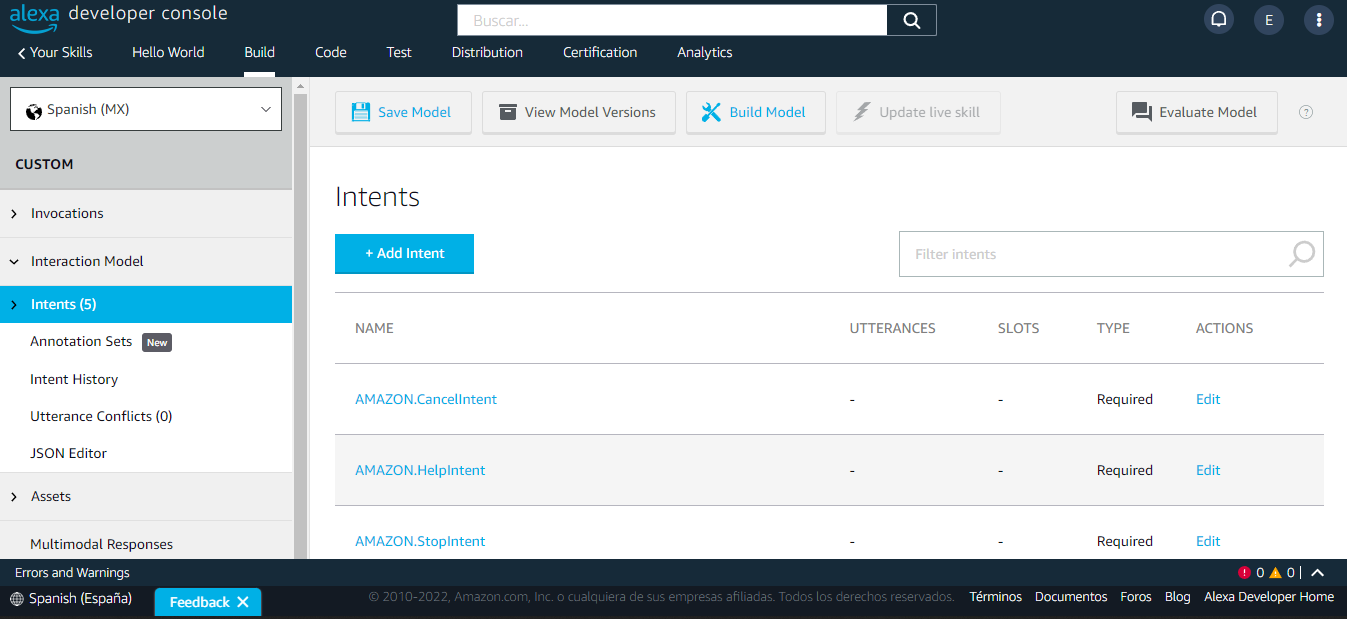
\includegraphics[width=0.70\textwidth]{Cap4/Figuras/Intenciones.png}
  \caption{Definición de intenciones de una skill.}
  \label{fig:46}
\end{figure}

Existen dos tipos de intenciones: predefinidas y personalizadas. Las intenciones predefinidas son acciones que ya se encuentran definidas y configuradas por la consola de desarrollo de Amazon.

% REFERENCIA
Entre las intenciones predefinidas, Amazon (2022k) define las siguientes:

\begin{itemize}
  \item \textbf{AMAZON.CancelIntent.} Es una intención definida para cancelar una acción en curso durante la skill.
  \item \textbf{AMAZON.HelpIntent.} Es una intención que puede ser configurada desde el código para ofrecer ayuda general sobre cómo usar la skill, con el fin de servir como guía al usuario.
  \item \textbf{AMAZON.StopIntent.} Es una intención que permite detener todas las acciones de una skill, terminando con el flujo y cerrando la skill.
  \item \textbf{AMAZON.NavigateHomeIntent.} Es una intención que se activa únicamente para dispositivos con pantalla, en la que se permite terminar la ejecución de una skill, devolviéndolos a la pantalla de inicio del dispositivo.
\end{itemize}

Existen otras intenciones predefinidas, que pueden ser agregadas manualmente desde la configuración de la consola de Amazon. Entre estas opciones se encuentran las siguientes intenciones:

\begin{itemize}
  \item \textbf{AMAZON.FallbackIntent.} Es una intención que permite dar alternativas para las expresiones que no hayan sido reconocidas por Alexa. Como respuesta de esta intención se puede dar detalle sobre la skill y cómo se puede interactuar con ella.
  \item \textbf{AMAZON.LoopOffIntent.} Permite al usuario la desactivación de un bucle para aquellas skills que desarrollan una funcionalidad de repetición. Por lo general. Por lo general esta intención se utiliza para skills que reproducen alguna lista de música o pistas.
  \item \textbf{AMAZON.LoopOnIntent.} Esta intención realiza la acción contraria a la intención anterior. Permite activar un bucle, generalmente para una lista de reproducción en skills que transmiten audio.
  \item \textbf{AMAZON.MoreIntent.} Es una intención que avanza el contenido actual para mostrar más contenido en dispositivos que tienen pantalla. Esta intención es similar al comportamiento de AMAZON.ScrollDownIntent y AMAZON.ScrollRightIntent.
  \item \textbf{AMAZON.NavigateSettingsIntent.} Esta intención funciona para dispositivos que cuentan con pantalla. Permite llevar al usuario a la pantalla de configuración del dispositivo y al salir regresará a la skill.
  \item \textbf{AMAZON.NextIntent.} Esta intención permite navegar a un siguiente elemento de una lista. En caso de tratarse de una skill que transmite audio, esta intención permite saltar a la siguiente reproducción.
  \item \textbf{AMAZON.NoIntent.} Facilita al usuario dar una respuesta negativa a preguntas del tipo $"$sí$"$ o $"$no$"$.
  \item \textbf{AMAZON.PageDownIntent.} Baja la vista a la siguiente pantalla de una interfaz en dispositivos que cuentan con pantalla.
  \item \textbf{AMAZON.PageUpIntent.} Sube la vista a una pantalla anterior de una interfaz en dispositivos que cuentan con pantalla.
  \item \textbf{AMAZON.PauseIntent.} Esta intención permite pausar el flujo de una skill, tal como pausar un videojuego o un audio en una lista de reproducción.
  \item \textbf{AMAZON.PreviousIntent.} Esta skill permite navegar a un elemento previo de una lista. En caso de tratarse de una skill que transmite audio, esta intención permite retroceder a la reproducción anterior.
  \item \textbf{AMAZON.RepeatIntent.} Permite repetir la última acción realizada por una skill.
  \item \textbf{AMAZON.ResumeIntent.} Reanuda o continua con alguna acción previamente puesta en pausa de una skill.
  \item \textbf{AMAZON.ScrollDownIntent.} Permite desplazar la interfaz hacia abajo de los dispositivos que cuentan con pantalla.
  \item \textbf{AMAZON.ScrollLeftIntent.} Permite desplazar la interfaz a la izquierda de los dispositivos que cuentan con pantalla.
  \item \textbf{AMAZON.ScrollRightIntent.} Permite desplazar la interfaz a la derecha de los dispositivos que cuentan con pantalla.
  \item \textbf{AMAZON.ScrollUpIntent.} Permite desplazar la interfaz hacia arriba de los dispositivos que cuentan con pantalla.
  \item \textbf{AMAZON.SelectIntent.} Permite al usuario indicar la selección de un elemento, por lo general de un listado de registros.
  \item \textbf{AMAZON.SendToPhoneIntent.} Se permite enviar información o resultados de una skill al teléfono a través de la app de Alexa en dispositivos móviles.
  \item \textbf{AMAZON.ShuffleOffIntent.} Permite desactivar el modo aleatorio en la skill. Por lo general, esta intención es usada para skills que transmiten audio en una lista de reproducción.
  \item \textbf{AMAZON.ShuffleOnIntent.} Permite activar el modo aleatorio de la skill. Generalmente para skills que transmiten audio en una lista de reproducción.
  \item \textbf{AMAZON.StartOverIntent.} Permite reiniciar una acción a un punto específico. Tal como reiniciar un juego o una pista de audio.
  \item \textbf{AMAZON.YesIntent.} Permite proporcionar una respuesta positiva para respuesta de preguntas del tipo $"$si$"$ o $"$no$"$.
\end{itemize}

Por otro lado, las intenciones personalizadas son intenciones que se crean manualmente desde la consola de desarrollo de Amazon, en la que se realizan las configuraciones necesarias para llevar a cabo acciones específicas fuera de las intenciones ya definidas por Amazon. Es recomendable que cuando se crea una nueva intención personalizada, esta debe nombrarse terminando con la palabra \textit{intent}. Por ejemplo, en la skill de ejemplo \textit{Comida Mexicana} podemos tener una intención que permita leer las instrucciones para preparar un platillo que pude ser llamada \textit{InstructionsIntent} o \textit{StartCookingIntent}.

%------------------------------------------------------------
%	Declaraciones
%------------------------------------------------------------

\subsubsection{Declaraciones}
\label{DeclaracionescapIV}

% REFERENCIA
Amazon (2022h), señala que las declaraciones o utterances son las diferentes frases que activan una intención. Cada intención tiene un apartado para definir las declaraciones como se muestra en la Figura \ref{fig:47}.

\begin{figure}[H]
% \begin{figure}
  \centering
  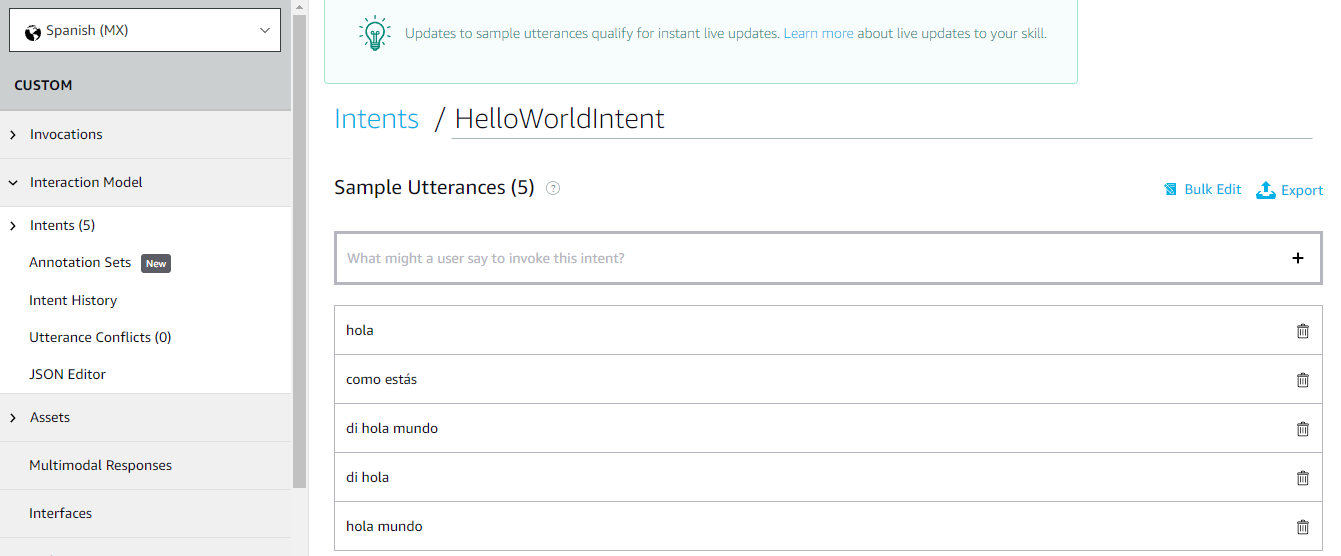
\includegraphics[width=0.70\textwidth]{Cap4/Figuras/Declaraciones.png}
  \caption{Definición de declaraciones de una intención de una skill.}
  \label{fig:47}
\end{figure}

Las intenciones predefinidas ya cuentan con declaraciones asociadas a su comportamiento, sin embargo, es posible definir declaraciones personalizadas extra en una invocación predefinida.

Por otro lado, cuando se crea una intención personalizada, es necesario definir al menos una declaración para poder activarla. Se recomienda fuertemente que las declaraciones estén diseñadas en el idioma en la que está definida la skill. Supongamos que tenemos la intención \textit{InstructionsIntent} que permite conocer las instrucciones para cocinar un platillo mexicano. Algunas de las declaraciones para poder activar la intención podrían ser las siguientes:

\begin{itemize}
  \item Dime las instrucciones de un platillo.
  \item Lee las instrucciones de un platillo.
  \item Comienza con el platillo.
  \item Quiero saber más información del platillo.
\end{itemize}

Este tipo de declaraciones puede ser aplicado tanto para invocaciones predefinidas como para invocaciones personalizadas. Sin embargo, existen otro tipo de declaraciones, las cuales permiten recabar información en forma de parámetros o argumentos dentro del mismo comando. A estos argumentos se les conoce como slots. Algunas de las declaraciones con slots para poder activar la intención \textit{InstructionsIntent} podrían ser las siguientes.

\begin{itemize}
  \item Dime las instrucciones para cocinar tacos al pastor.
  \item Comienza a cocinar pozole.
  \item Quiero aprender a cocinar alambre de bistec.
\end{itemize}

En las declaraciones anteriores, se solicita información específica que pasa por medio de argumentos, tal como tacos al pastor, pozole o alambre de bistec. Como estos datos son parámetros en la declaración, la estructura con slots de las mismas declaraciones se vería como sigue:

\begin{itemize}
  \item Dime las instrucciones para cocinar \{nombrePlatillo\}.
  \item Comienza a cocinar \{nombrePlatillo\}.
  \item Quiero aprender a cocinar \{nombrePlatillo\}.
\end{itemize}

En donde la variable \textit{nombrePlatillo} corresponde a un valor específico.

% REFERENCIA
Amazon (2022h) señala que una declaración se forma de la estructura descrita en la Figura \ref{fig:48}.

\begin{figure}[H]
% \begin{figure}
  \centering
  
\includegraphics[width=0.70\textwidth]{Cap4/Figuras/Estructura de Declaraciones.jpg}
  \caption{Estructura de una declaración o utterance. Amazon (2022h).}
  \label{fig:48}
\end{figure}

Donde:

\begin{itemize}
  \item \textbf{SearchAction.} Es un objeto que realiza la búsqueda de una acción que el usuario quiere ejecutar.
  \item \textbf{object.} Es un objeto en el que se identifican las entidades involucradas en una declaración y con el que se puede operar.
  \item \textbf{attributes.} Son aquellos valores que pasan por medio de uno o más slots. La forma en la que se accede a estos valores es por medio de object.
\end{itemize}

%------------------------------------------------------------
%	Slots
%------------------------------------------------------------

\subsubsection{Slots}
\label{SlotscapIV}

% REFERENCIA
Como se comentó anteriormente, Amazon (2022i) define los slots como argumentos que son proporcionados en una declaración. Estos argumentos son una herramienta útil para recabar información de diferentes tipos.

La configuración y definición de los slots usados en las declaraciones de una intención se encuentra en la sección de construcción de una skill, tal como se muestra en la Figura \ref{fig:49}.

\begin{figure}[H]
% \begin{figure}
  \centering
  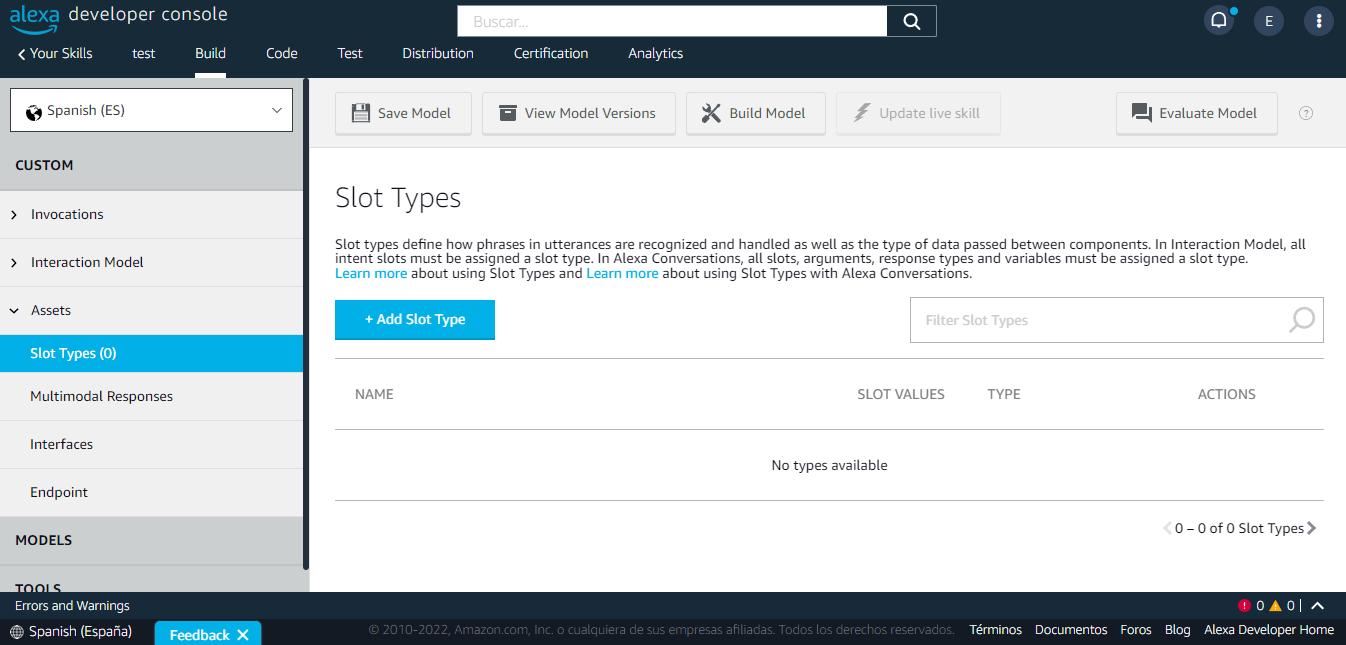
\includegraphics[width=0.70\textwidth]{Cap4/Figuras/SlotTypes.png}
  \caption{Definición de slots para las declaraciones de una skill.}
  \label{fig:49}
\end{figure}

Existen dos tipos de slots: slots predefinidos y slots personalizados. A su vez, los slots predefinidos se dividen en dos categorías. Por una parte, existen slots que reconocen valores en una lista de sugerencias que puede ser extendida por el desarrollador. Por otra parte, se tienen slots que convierten un dato en información específica que no está definida en una lista, por lo que estos no pueden ser extendidos por el desarrollador.

% REFERENCIA
Amazon (2022i) señala que entre los slots predefinidos se encuentran los siguientes:

\begin{itemize}
  \item \textbf{AMAZON.Actor.} Es un slot que almacena una lista con nombres de actores y actrices.
  \item \textbf{AMAZON.Airline.} Contiene una lista con gran variedad de nombres de aerolíneas.
  \item \textbf{AMAZON.Airport.} Almacena una gran variedad de nombres de aeropuertos.
  \item \textbf{AMAZON.Anaphor.} Contiene palabras que representan una anáfora. Tales como $"$este$"$, $"$eso$"$, $"$esa$"$, etc.
  \item \textbf{AMAZON.Animal.} Lista con una gran variedad de nombres de animales.
  \item \textbf{AMAZON.Artist.} Lista con una gran variedad de nombres completos de artistas.
  \item \textbf{AMAZON.Book.} Listado de algunos títulos de libros.
  \item \textbf{AMAZON.City.} Provee un listado de ciudades comúnmente usadas localmente, según la configuración de idioma en que está desarrollada la skill.
  \item \textbf{AMAZON.Color.} Listado con los nombres de los colores.
  \item \textbf{AMAZON.Corporation.} Listado con el nombre completo de varias corporaciones.
  \item \textbf{AMAZON.Country.} Listado del nombre de los países o regiones del mundo.
  \item \textbf{AMAZON.CreativeWorkType.} Listado de palabras usadas en trabajos creativos, tal como $"$canción$"$, $"$show$"$, $"$escenario$"$, etc.
  \item \textbf{AMAZON.DayOfWeek.} Listado de los días de la semana basados en el calendario.
  \item \textbf{AMAZON.FictionalCharacter.} Listado de nombres de personajes ficticios de libros, películas, televisión, entre otros.
  \item \textbf{AMAZON.FirstName.} Listado de gran cantidad de nombres usados localmente, por ejemplo, los nombres más usados por hablantes mexicanos para una skill configurada con localidad en México.
  \item \textbf{AMAZON.Food.} Listado de nombres de diferentes platillos.
  \item \textbf{AMAZON.Genre.} Listado de diferente tipo de géneros que describen música, libros, espectáculos de televisión, entre otros.
  \item \textbf{AMAZON.Language.} Listado con diferentes idiomas, tal como español, inglés, chino, etc.
  \item \textbf{AMAZON.Month.} Listado del nombre de los meses en el calendario.
  \item \textbf{AMAZON.Movie.} Listado de gran variedad de películas.
  \item \textbf{AMAZON.MusicAlbum.} Listado de nombres de álbumes musicales.
  \item \textbf{AMAZON.MusicGroup.} Listado del nombre de diferentes grupos musicales, tales como bandas, orquestas, coros e incluso artistas independientes.
  \item \textbf{AMAZON.Musician.} Listado del nombre completo de algunos músicos.
  \item \textbf{AMAZON.MusicRecording.} Listado del nombre de varias canciones grabadas.
  \item \textbf{AMAZON.Person.} Listado de nombres completos de personas reales o ficticias.
  \item \textbf{AMAZON.RadioChannel.} Listado del nombre de diferentes canales o estaciones de radio.
  \item \textbf{AMAZON.Region.} Provee una lista de países y regiones generalmente usados por los hablantes de la localidad de la skill.
  \item \textbf{AMAZON.RelativePosition.} Provee un listado de palabras que reconocen la posición relativa de un elemento en una lista, tal como $"$primero$"$ o $"$último$"$.
  \item \textbf{AMAZON.Room.} Listado del nombre de diferentes habitaciones o cuartos de una casa y otras edificaciones.
  \item \textbf{AMAZON.Sport.} Listado con el nombre de diferentes deportes.
  \item \textbf{AMAZON.StreetName.} Listado con el nombre de diferentes calles y avenidas.
  \item \textbf{AMAZON.TVSeries.} Listado con una gran cantidad de títulos y nombres de series de televisión.
  \item \textbf{AMAZON.VideoGame.} Listado con el nombre de varios videojuegos.
  \item \textbf{AMAZON.VisualModeTrigger.} Listado de palabras relacionadas a la espera de una respuesta visual, tal como $"$muestra$"$ o $"$despliega$"$.
\end{itemize}

Cabe mencionar que los valores proporcionados en los slots anteriores podrían no considerar datos específicos que requiere una skill. Es por ello que la consola de Amazon provee la posibilidad de extender los valores de estas listas, definiendo aquellos valores que también puede considerar.

Sin embargo, se cuentan con los slots predefinidos que no se basan en un listado de palabras o definiciones, sino que transforman una entrada a un tipo de valor específico, tal como los números. Entre estos slots se encuentran los siguientes:

\begin{itemize}
  \item \textbf{AMAZON.DATE.} Convierte palabras que indican una fecha, tales como “hoy”, “mañana”, “agosto” y los convierte a un formato de fecha, tal como “2015-07-00T9”.
  \item \textbf{AMAZON.DURATION.} Convierte palabras que indican una duración, tal como “una hora”, “dos semanas”, y los convierte a una duración numérica del tipo “PT5M”.
  \item \textbf{AMAZON.FOUR\_DIGIT\_NUMBER.} Convierte palabras a un número de cuatro dígitos, por ejemplo la frase “cinco, cuatro, tres, dos” se convierte a un valor numérico como “5432”.
  \item \textbf{AMAZON.NUMBER.} Convierte palabras que representan un dígito en un número, tal como “seis” a “6”.
  \item \textbf{AMAZON.Ordinal.} Convierte palabras que representan números ordinales en dígitos, tal como “tercero” a “3”.
  \item \textbf{AMAZON.PhoneNumber.} Convierte palabras que representan un número telefónico a un dígito con representación a números de teléfono locales, nacionales e internacionales.
  \item \textbf{AMAZON.SearchQuery.} Convierte una palabra o frase en una oración que podría ser ingresada en un motor de búsqueda estándar.
  \item \textbf{AMAZON.TIME.} Convierte palabras que indican tiempo, tal como “seis de la mañana” y los convierte a un valor con formato horario como “06:00” con un tiempo de 24 horas.
\end{itemize}

Sin embargo,  a pesar de la gran variedad de slots predefinidos en la consola de Amazon, cabe la posibilidad de que se necesite un slot con valores específicos para alguna skill. A estos slots se les conoce como slots personalizados, en los que se determinan los valores que puede reconocer.

% REFERENCIA
Amazon (2022i) señala que los valores definidos para un slot personalizado puede ser cualquier palabra que pueda ser pronunciada por un usuario. De lo contrario, es muy probable que no se pueda reconocer alguna palabra que no se encuentre definida en un diccionario del idioma en que está configurada la skill.

Es importante considerar que las frases que contienen acrónimos, se deben definir en los valores del slot en letras mayúsculas o en letras minúsculas seguidos de un punto. Por ejemplo, si se requiere tener como valor el acrónimo CDMX, este debe estar definido como $"$CDMX$"$ o $"$c. d. m. x.$"$ como valor del slot.

Al momento de crear un slot, cabe la posibilidad de agregarle sinónimos y un identificador, tal como se muestra en la Figura \ref{fig:410}. Los sinónimos pueden ser usados como alternativas al valor original de un elemento de la lista de valores.

\begin{figure}[H]
% \begin{figure}
  \centering
  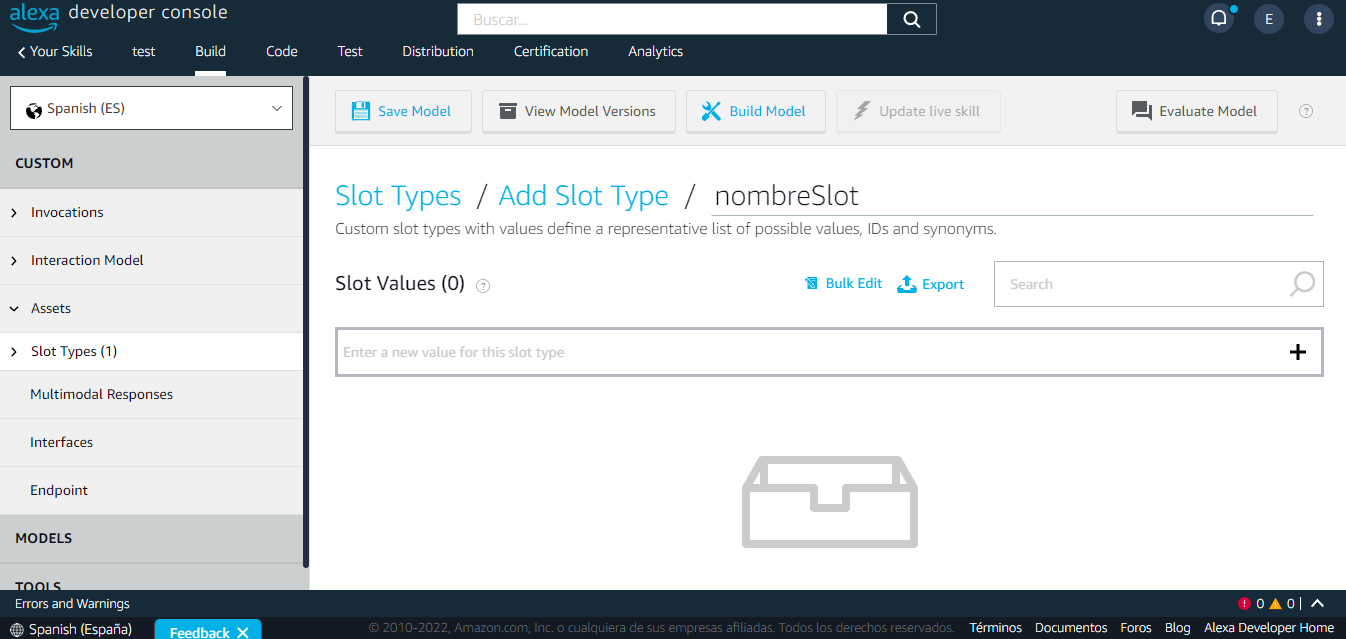
\includegraphics[width=0.70\textwidth]{Cap4/Figuras/SlotTypesCreation.png}
  \caption{Ejemplo de sinónimos de un slot.}
  \label{fig:410}
\end{figure}

%------------------------------------------------------------
%	Función Lambda
%------------------------------------------------------------

\subsubsection{Función Lambda}
\label{FuncionLambdacapIV}

% REFERENCIA
El código donde se implementan las invocaciones de la skill se definen en una función llamada función Lambda. Amazon (2022j) señala que existen dos formas de crear una función Lambda: la primera forma consiste en hospedar el código en los servicios de la consola de desarrollo de Alexa, en la que se permite desarrollar en los lenguajes de programación Python y Node.js; la segunda forma consiste en hospedar la función Lambda en el servicio de Amazon Web Services (AWS), llamado AWS Lambda, en la que se da la posibilidad de programar en los lenguajes de programación Node.js, Java, Python, Go, Ruby y C\#.

La función lambda que se hospeda en la consola de desarrollo de Amazon, se encuentra definida en la sección llamada Code del flujo de implementación de una skill. Para el lenguaje de programación Node.js, se encuentra definida en el archivo index.js, dentro del directorio llamado lambda. Mientras que para el lenguaje de programación Python, se encuentra en el archivo llamado \textit{lambda\_function.py}, dentro del directorio llamado lambda.

Esta función se encuentra predefinida en la sección de código, tal como se muestra en la Figura \ref{fig:411}.

\begin{figure}[H]
% \begin{figure}
  \centering
  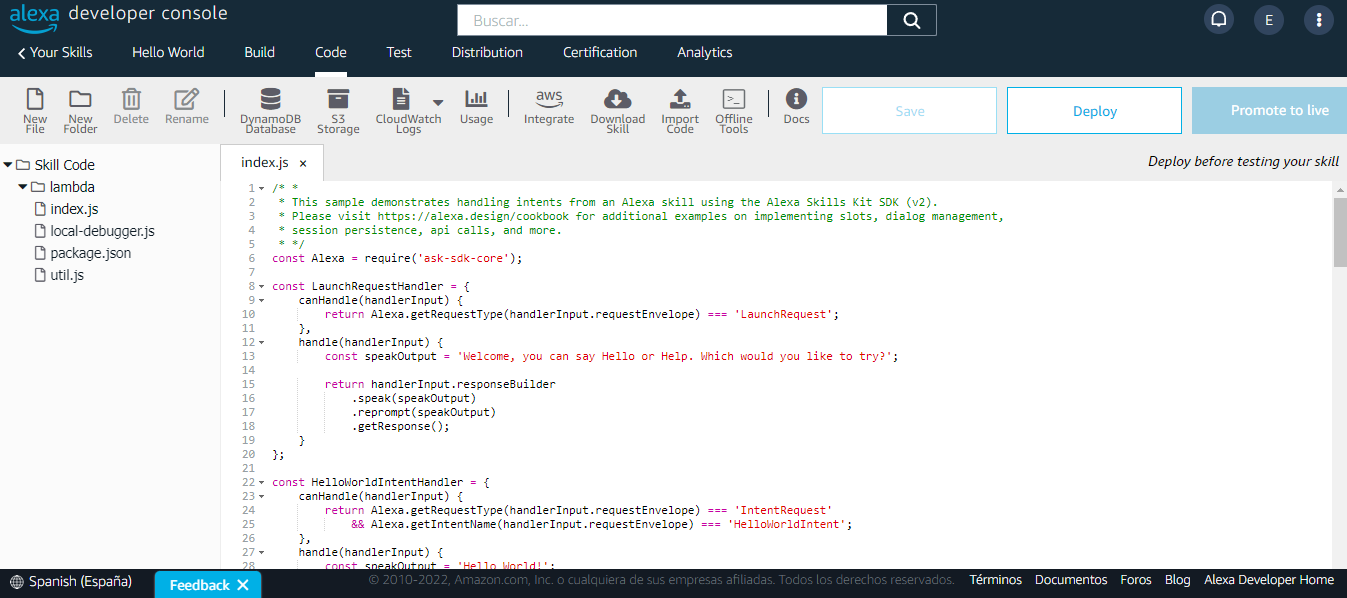
\includegraphics[width=0.70\textwidth]{Cap4/Figuras/Funcionlambda.png}
  \caption{Declaración de la función Lambda de una skill.}
  \label{fig:411}
\end{figure}

La función importa por omisión la biblioteca llamada \textit{ask\_sdk\_core}, la cual contiene funcionalidades para poder programar las acciones básicas en Alexa, tales como las siguientes:

\begin{itemize}
  \item El constructor de skills.
  \item El controlador de solicitudes definidas para el reconocimiento de las intenciones por reconocimiento por voz.
  \item El lanzador de inicio de ejecución de la skill, con el reconocimiento del nombre de invocación de la skill.
  \item El reconocedor de nombres de las intenciones definidas de la skill.
  \item El constructor de respuestas de las intenciones de la skill.
\end{itemize}

Cabe mencionar que existen más propiedades que pueden ser importadas manualmente para implementar funcionalidades extra.

La función contiene un conjunto de controladores de solicitudes, los cuales se denominan \textit{Handlers}. Estos permiten definir el comportamiento específico de una intención, con el que se provee una respuesta a la acción por medio del constructor de respuestas.

Existen dos tipos de Handlers: los handlers que están a la espera de solicitudes de tipo LaunchRequest y los que están a espera de solicitudes IntentRequest.

\begin{itemize}
  \item \textbf{LaunchRequest.} Existe sólo un handler con este tipo de solicitud en la Lambda. Este handler se ejecuta cuando un usuario dice un comando de activación de la skill. Da como respuesta la bienvenida o introducción general a la skill, así como sugerencias a un comando de inicio para seguir el flujo. De manera predefinida, al crear una nueva skill con Python, la consola de desarrollo de Alexa genera el siguiente ejemplo de un handler con solicitud de tipo LaunchRequest.
  \begin{tcolorbox}[colback=white!25!white,colframe=blue]
    \begin{minted}{python}
class LaunchRequestHandler(AbstractRequestHandler):
  """Handler for Skill Launch."""
  def can_handle(self, handler_input):
    # type: (HandlerInput) -> bool
  
    return ask_utils.is_request_type("LaunchRequest")(handler_input)
  
  def handle(self, handler_input):
    # type: (HandlerInput) -> Response
    speak_output = "Welcome, you can say Hello or Help."+
      "Which would you like to try?"
  
    return (
      handler_input.response_builder
        .speak(speak_output)
        .ask(speak_output)
        .response
    )
    \end{minted}
  \end{tcolorbox}
  \item \textbf{IntentRequest.} Son aquellos handlers que se ejecutan cuando una intención es activada. Este tipo de handlers reciben un parámetro adicional, que corresponde al nombre exacto de la intención que se quiere ejecutar. De manera predefinida, al crear una nueva skill con Python, la consola de desarrollo de Alexa genera el siguiente ejemplo de un IntentRequest.
  \begin{tcolorbox}[colback=white!25!white,colframe=blue]
    \begin{minted}{python}
class HelloWorldIntentHandler(AbstractRequestHandler):
  """Handler for Hello World Intent."""
  def can_handle(self, handler_input):
    # type: (HandlerInput) -> bool
    return ask_utils.is_intent_name("HelloWorldIntent")(handler_input)

  def handle(self, handler_input):
    # type: (HandlerInput) -> Response
    speak_output = "Hello World!"

    return (
      handler_input.response_builder
        .speak(speak_output)
        # .ask("add a reprompt if you want to keep the session
        # open for the user to respond")
        .response
    )
    \end{minted}
  \end{tcolorbox}
\end{itemize}

Los slots que intervienen en un handler también se transmiten como parámetros para poder ser accesibles dentro de la definición de la función que lo implementa. A estos se accede de forma diferente, dependiendo del lenguaje de programación. Para el caso de Python se usa la siguiente sintaxis.

\begin{tcolorbox}[colback=white!25!white,colframe=blue]
  \begin{minted}{python}
handler_input.request_envelope.request.intent.slots['slotName']
  \end{minted}
\end{tcolorbox}

Donde \textit{slotName} corresponde al nombre del slot que se quiere recuperar. Este ya cuenta con todas las propiedades definidas en el proceso de definición del slot.

Es importante mencionar que estos handlers pueden definirse en el archivo pero no son reconocidos automáticamente por el constructor de la skill. Estos deben ser agregados como parámetros a la función de definición de handlers para cambiar a un estado de activación para el reconocimiento por voz de los comandos asociados. La sintaxis para activar los handlers en Python de una skill se presenta a continuación.

\begin{tcolorbox}[colback=white!25!white,colframe=blue]
  \begin{minted}{python}
sb = SkillBuilder()
sb.add_request_handler(LaunchRequestHandler())
sb.add_request_handler(Intent1Handler())
sb.add_request_handler(Intent2Handler())
…
sb.add_request_handler(IntentNHandler())
  \end{minted}
\end{tcolorbox}

%------------------------------------------------------------
%	Simulador de Alexa
%------------------------------------------------------------

\subsubsection{Simulador de Alexa}
\label{SimuladorcapIV}

% REFERENCIA
Amazon (2022l) señala que existe una página en la que se pueden realizar pruebas del funcionamiento de la skill, para corroborar su correcto comportamiento con el reconocimiento de voz, intenciones, declaraciones, slots, respuestas progresivas y la resolución de entidades. Amazon (2022l) recomienda que antes de realizar pruebas a la skill, se configuren las características mínimas requeridas para su funcionamiento en la consola de desarrollo, tales como la definición de intenciones, la configuración de declaraciones y la implementación del código.

El apartado llamado \textit{Test}, provee tres formas diferentes para poder realizar pruebas en una skill. Cada una de estas formas está enfocada a características específicas como las siguientes:

\begin{itemize}
  \item \textbf{Simulador de Alexa.} Provee la posibilidad de realizar pruebas en una skill por medio de texto y voz, además, provee las herramientas necesarias para manejar la skill como si se estuviera utilizando un dispositivo con el servicio de Alexa integrado.
  \item \textbf{Manual de JSON.} Permite ingresar objetos con el formato JSON directamente a las solicitudes de la skill, así como ver la respuesta JSON que la skill lanza como respuesta. Este manual es muy útil para mandar información a lambdas de AWS por medio de endpoints, que son URLs de puntos de entrada para un servicio de AWS, hospedados en regiones específicas.
  \item \textbf{Voz y tonos.} Alexa permite dar respuestas con tonos diferentes a la tonalidad habitual, por medio de un mecanismo llamado Speech Synthesis Markup Language (SSML). El SSML permite que Alexa exprese frases con diferentes tonos, tales como emoción, tristeza, susurros, pausas largas, entre otros. El paso de datos por archivos con el formato SSML permite interactuar con la forma en que Alexa podría dar diferentes respuestas.
\end{itemize}

% REFERENCIA
Amazon (2022m) menciona que el simulador de Alexa también permite tener una vista previa a los servicios de Alexa Presentation Language (APL), que permite tener una interfaz gráfica para aquellos dispositivos que cuenten con una pantalla. En esa configuración se puede observar cómo se vería el resultado final en diferentes dispositivos con Alexa integrada que cuentan con pantalla, tales como dispositivos Hub Round Small, Hub Landscape Small, Hub Landscape Medium, Hub Landscape Large, .Hub Landscape Extra Large, Hub Portrait Medium, TV Landscape Extra Large, Mobile Small, Mobile Medium y Mobile Large.

% REFERENCIA
Amazon (2022m) señala que es necesario cumplir ciertos requisitos previos para habilitar los test en el simulador de Alexa.

\begin{itemize}
  \item Sólo sirve para skills personalizadas.
  \item Se debe configurar un endpoint válido para la skill. Por lo que es importante implementar un punto de finalización para el término de la ejecución de la skill.
  \item La skill se debe habilitar dentro de la página de Test.
  \item Para skills de video, es necesario habilitar la skill en la aplicación de Alexa, completando la información requerida.
\end{itemize}

Así mismo, es posible habilitar otras herramientas para realizar pruebas sobre la skill desde el simulador de Alexa. Entre estas se encuentran las siguientes opciones.

\begin{itemize}
  \item \textbf{I/O de la skill.} Permite visualizar las cargas útiles sobre las solicitudes y respuestas de Alexa en formato JSON. Se muestran las solicitudes hechas por el usuario y la respuesta de diálogo con toda su configuración en un objeto en formato JSON.
  \item \textbf{Visualizador de dispositivos con pantalla.} Se muestra un aproximado de cómo se vería la interfaz gráfica en pantalla por medio del servicio de APL.
  \item \textbf{Registros de dispositivos.} Permite visualizar los eventos enviados a Alexa, así como las directivas en cada interacción con la skill.
  \item \textbf{Alexa Smart Home (Beta).} permite visualizar los eventos de tipo ChangeReport que la skill envía como enlaces a eventos de Alexa. Esta funcionalidad sólo está disponible para skills enfocadas a hogares inteligentes.
\end{itemize}

% REFERENCIA
Finalmente, Amazon (2022m) señala que el simulador de Alexa provee un sistema de depuración de intenciones, habilitando la funcionalidad llamada Device Log, en la que se muestran todas las intenciones devueltas por la skill en formato JSON. Esta forma de depuración es útil para resolver expresiones y casos no previstos en las intenciones definidas.

El simulador de Alexa se encuentra en la sección de pruebas de la skill, tal como se muestra en la Figura \ref{fig:412}.

\begin{figure}[H]
% \begin{figure}
  \centering
  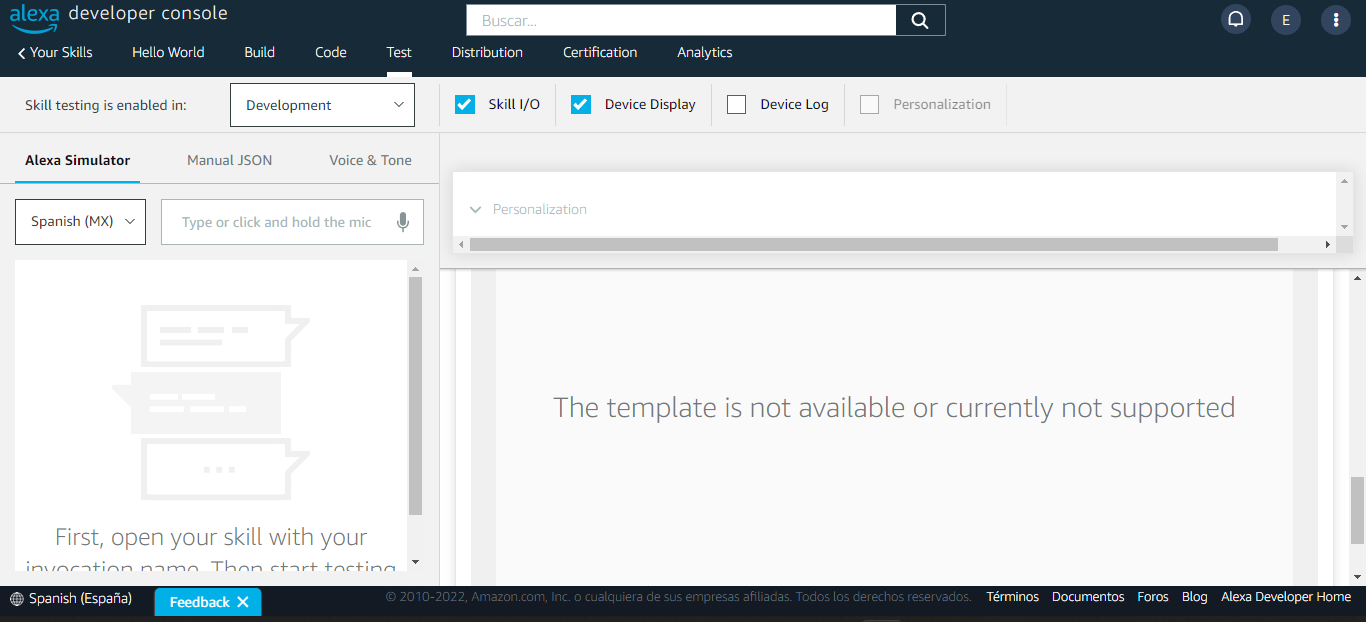
\includegraphics[width=0.70\textwidth]{Cap4/Figuras/Simulador.png}
  \caption{Simulador de Alexa para las pruebas de una skill.}
  \label{fig:412}
\end{figure}

%------------------------------------------------------------
%	Análisis del problema
%------------------------------------------------------------

\section{Análisis del problema}
\label{AnalisisProblemacapIV}

El análisis del problema es una etapa fundamental para identificar las oportunidades de mejora que pueden considerarse para atacar un problema de una forma efectiva, así como el desarrollo de una solución que satisfaga las necesidades del usuario, en este análisis, basados en el diseño centrado en el usuario.

A continuación se presenta una descripción que detalla la identificación de los principales problemas presentados durante la búsqueda e investigación de información, así como las oportunidades de mejora encontradas en cada paso del Modelo Gavilán.

%------------------------------------------------------------
%	Identificación del problema
%------------------------------------------------------------

\subsection{Identificación del problema}
\label{IdentificacionProblemacapIV}

En el Diplomado Internacional de Innovación en la Docencia Universitaria del año 2020, se consideraron diferentes aspectos y características sobre los mayores problemas con los que se enfrentan los alumnos al momento de realizar una investigación.

Como parte de las actividades del diplomado, los profesores expresaron diferentes puntos de vista sobre la deficiencia del proceso de búsqueda de información que generalmente cometen los alumnos. Muchos de los profesores comparten puntos similares que notaron durante el análisis de la actividad, entre los que destacan los siguientes:

\begin{itemize}
  \item Gran parte de la investigación se basa en un proceso de copiar y pegar información.
  \item Dado que la información, por lo general se copia y pega, no se analiza el contenido de la investigación.
  \item No se establece un objetivo para la investigación, por lo que se busca directamente el contenido, omitiendo puntos relevantes e insertando información que no forma parte de los límites de la investigación.
  \item La mayor fuente de información que se utiliza es la Internet. Donde se selecciona, por lo general, las primeras páginas que resultan de la búsqueda. Cabe resaltar que estas páginas no necesariamente son confiables por estar en las primeras posiciones de la búsqueda.
  \item Generalmente se selecciona la fuente de información que describa la mayor cantidad de información sobre el contenido solicitado en la investigación.
  \item El proceso que siguen los alumnos para determinar si la información es confiable, consiste en buscar información y mientras más aparezca un mismo dato en diferentes fuentes, más confiable es.
  \item Cuando se utiliza un navegador por Internet, se buscan las respuestas tal cual como se solicitan.
  \item No se utilizan fuentes bibliográficas ni referencias que sustenten el contenido de la investigación.
  \item Por lo general, los alumnos buscan en internet una búsqueda sencilla y apresurada. El principal objetivo de los alumnos durante una investigación es encontrar contenido lo más pronto posible, sin importar tanto la información.
\end{itemize}

Por otra parte, se realizó una investigación para conocer el proceso que realizan los estudiantes de licenciatura de la Facultad de Ciencias en los primeros semestres de la carrera, con el fin de encontrar los problemas durante el proceso.

La investigación con los estudiantes de los primeros semestres de licenciatura arrojaron resultados similares a los problemas encontrados con los alumnos de preparatoria, entre ellos se encuentran los siguientes:

\begin{itemize}
  \item Se consultan los primeros resultados del motor de búsqueda de un navegador.
  \item Se realiza la búsqueda a partir de una pregunta o frase que involucre todo el tema, sin delimitar ni analizar la información.
  \item Al encontrar la información más relevante, se detiene la investigación.
  \item En ocasiones, se busca información en diferentes fuentes, donde se pueden encontrar datos y contenido repetido.
  \item La base de la búsqueda está centralizada en copiar y pegar información, sin pasar por un proceso de análisis del contenido.
\end{itemize}

Según las descripciones dadas por los resultados de las actividades del Diplomado Internacional de Innovación en la Docencia Universitaria, se encontró un patrón general sobre el proceso de investigación que habitualmente realizan los estudiantes. Este proceso se menciona a continuación:

\begin{itemize}
  \item Si la investigación cuenta con preguntas específicas, estas se buscan en el navegador, tal cual como se solicita en la asignación.
  \item En caso de no haber preguntas específicas definidas, se busca de forma general el tema de la investigación.
  \item La mayor parte de los alumnos utiliza Internet para realizar una investigación. Los primeros resultados que arroja el motor de búsqueda son aquellos que se seleccionan principalmente para extraer contenido.
  \item El contenido de la página se lee de forma muy general. Si el alumno determina que el contenido cubre todos los aspectos y datos solicitados en la investigación, copia y pega el contenido.
  \item Si la fuente de información no contiene los datos requeridos, se procede a buscar en las siguientes opciones de búsqueda que aparecen primero en el buscador y se realiza el mismo proceso del punto anterior.
  \item Por lo general, cuando los extractos de información contienen los datos requeridos, se termina la investigación, sin comentar o incluir comentarios que concluyan la investigación.
  \item Un factor importante sobre la extensión de la investigación es la cantidad de párrafos o páginas extraídos. Los alumnos consideran que entre más información se incluya en la investigación, mejor será la calidad del trabajo.
\end{itemize}

%------------------------------------------------------------
%	Comparación con el Modelo Gavilán
%------------------------------------------------------------

\subsection{Comparación con el Modelo Gavilán}
\label{ComparacionModeloGavilancapIV}

Una de las actividades que realizaron algunos profesores como parte del Diplomado Internacional Innovación en la Docencia Universitaria, fue mostrar la comparación entre los pasos del Modelo Gavilán y el proceso habitual que aplican los alumnos para completar un trabajo de búsqueda de información. En esta comparación se pueden identificar los pasos en los que los alumnos tienen mayor dificultad para realizar la investigación o que omiten por completo.

A continuación se muestra la Tabla \ref{tab:t42} con la comparación entre los pasos del Modelo Gavilán y los pasos que siguen los alumnos, según los resultados de los profesores del Diplomado Internacional de Innovación en la Docencia Universitaria y los resultados concluidos con el análisis con los alumnos de licenciatura.

\begin{table}[H]
  \begin{center}
    \begin{tabular}{ | p{2cm} | p{7cm} | p{7cm} | }
      \hline
      ETAPA & MODELO GAVILÁN & INVESTIGACIÓN DE ALUMNOS \\ \hline
      1 & 
      DEFINIR EL PROBLEMA DE INFORMACIÓN Y QUÉ SE NECESITA INDAGAR PARA RESOLVERLO
      \begin{itemize}
        \item Subpaso 1a: Plantear una Pregunta Inicial.
        \item Subpaso 1b: Analizar la Pregunta Inicial.
        \item Subpaso 1c: Construir un Plan de Investigación.
        \item Subpaso 1d: Formular Preguntas Secundarias.
        \item Subpaso 1e: Evaluación del Paso 1.
      \end{itemize}
      & 
      IDENTIFICAR LA INFORMACIÓN QUE SE NECESITA INVESTIGAR
      \begin{itemize}
        \item Identificar palabras o preguntas clave que respondan a la solicitud de la investigación
        \item Formular una pregunta o una frase utilizando las palabras clave identificadas.
      \end{itemize}
      \\ \hline
      2 & 
      BUSCAR Y EVALUAR FUENTES DE INFORMACIÓN
      \begin{itemize}
        \item Subpaso 2a: Identificar y seleccionar las fuentes de información más adecuadas.
        \item Subpaso 2b: Acceder a las fuentes de información seleccionadas.
        \item Subpaso 2c: Evaluar las fuentes encontradas.
        \item Subpaso 2d: Evaluación Paso 2.
      \end{itemize}
      & 
      IDENTIFICAR LAS FUENTES DE INFORMACIÓN MÁS APROPIADAS
      \begin{itemize}
        \item Seleccionar un conjunto de fuentes donde posiblemente se encuentre la información requerida.
        \begin{itemize}
          \item Sitios Web (100\%)
          \item Libros (75\%)
          \item Libros digitales (50\%)
          \item Youtube (50\%)
        \end{itemize}
      \end{itemize}
      \\ \hline
      3 & 
      ANALIZAR LA INFORMACIÓN
      \begin{itemize}
        \item Subpaso 3a: Elegir la información más adecuada para resolver las Preguntas Secundarias
        \item Subpaso 3b: Leer, entender, comparar, y evaluar la información seleccionada
        \item Subpaso 3c: Responder las Preguntas Secundarias
        \item Subpaso 3d: Evaluación Paso 3
      \end{itemize}
      & 
      OBTENCIÓN DE INFORMACIÓN
      \begin{itemize}
        \item Destacar la información más importante encontrada en las primeras sugerencias de un navegador.
        \item Se obtiene únicamente la información más clara y simple que responda a lo solicitado en la investigación.
      \end{itemize}
      \\ \hline
      4 & 
      SINTETIZAR LA INFORMACIÓN Y UTILIZARLA
      \begin{itemize}
        \item Subpaso 4a: Resolver la Pregunta Inicial
        \item Subpaso 4b: Elaborar un producto concreto
        \item Subpaso 4c: Comunicar los resultados de la investigación
        \item Subpaso 4d: Evaluación del Paso 4 y del Proceso
      \end{itemize}
      & 
      PROFUNDIZAR EN EL TEMA
      \begin{itemize}
        \item A forma de complemento, se profundiza el tema con ejemplos y otras definiciones, dependiendo de los siguientes factores
        \begin{itemize}
          \item Interés del alumno por el tema.
          \item Si la cantidad de información es poca.
        \end{itemize}
      \end{itemize}
      \\ \hline
    \end{tabular}
    \caption{Pasos del Modelo Gavilán y pasos que siguen los alumnos.}
    \label{tab:t42}
  \end{center}
\end{table}

De la comparación presentada en la tabla anterior, se puede observar que muchos puntos que define el Modelo Gavilán son omitidos o realizados de forma incompleta durante una investigación habitual de los alumnos de nivel bachillerato y de primeros semestres de licenciatura.

\begin{itemize}
  \item \textbf{Etapa 1.} Los subpasos propuestos en la primera fase del Modelo Gavilán tienen como objetivo delimitar la búsqueda de información. En el caso del proceso de investigación de los estudiantes, no se delimita el tema y se realiza una búsqueda más directa sin un proceso de análisis, por lo que la investigación podría omitir o tener información de más.
  \item \textbf{Etapa 2.} Los subpasos propuestos en la segunda fase del Modelo Gavilán tienen como objetivo indagar en las fuentes de información para encontrar contenido útil. Sin embargo, en una investigación habitual de los alumnos, se buscan fuentes de información donde extraer contenido, sin analizarlas. Entre las fuentes más usadas para extraer información se encuentran las siguientes.
  \begin{itemize}
    \item El 100\% de los alumnos en las pruebas usan sitios web.
    \item El 75\% de los alumnos en las pruebas usan libros.
    \item El 50\% de los alumnos en las pruebas usan libros digitales.
    \item El 50\% de los alumnos en las pruebas usan recursos visuales como Youtube.
  \end{itemize}
  \item \textbf{Etapa 3.} Los subpasos propuestos en la tercera fase del Modelo Gavilán tienen como objetivo analizar la información para determinar si es útil, de calidad, confiable, entre otros. En una investigación habitual, la información extraída no pasa por un proceso de análisis para determinar si cumple con las características mencionadas anteriormente. Por lo general, se extrae información de las primeras recomendaciones dadas por un navegador, ya que los alumnos afirman que las primeras recomendaciones son más confiables.
  \item \textbf{Etapa 4.} Los subpasos propuestos en la cuarta fase del Modelo Gavilán tienen como objetivo sintetizar y organizar la información. En una investigación habitual no se realiza un proceso de síntesis, sino de recopilación de toda la información extraída en un documento. Por lo general, las referencias bibliográficas no son incluidas en el trabajo final de los alumnos que participaron en la prueba.
\end{itemize}

%------------------------------------------------------------
%	Análisis del usuario y la tarea
%------------------------------------------------------------

\section{Análisis del usuario y la tarea}
\label{AnalisisUsuariocapIV}

Una vez identificados los puntos críticos del problema que suelen tener los estudiantes al momento de realizar una investigación, se dio paso a crear herramientas que sirvan como apoyo para conocer de mejor forma a los usuarios.

Con el fin de seguir la metodología de diseño centrado en el usuario, se crearon dos herramientas: modelo Persona y el Customer Journey Map. Como se mencionó anteriormente, el modelo Persona permite conocer las necesidades, experiencias y comportamientos de los usuarios para generar empatía con un producto, en este caso, con la skill desarrollada para atacar el problema de búsqueda de información.

Por otro lado, el Customer Journey Map tiene el objetivo de examinar la historia de cómo un usuario se relaciona con un servicio a lo largo del tiempo. En este caso, se orienta a conocer el proceso de investigación que siguen los usuarios, según los resultados de las investigaciones realizadas en el Diplomado Internacional de Innovación en la Docencia Universitaria y la investigación realizada con los estudiantes de primeros semestres de licenciatura de la Facultad de Ciencias.

%------------------------------------------------------------
%	Diseño de Persona para la skill
%------------------------------------------------------------

\subsection{Diseño de Persona para la skill}
\label{DisenioPersonacapIV}

Con el fin de conocer las necesidades, objetivos y características particulares de los alumnos, se crearon dos modelos Persona. El primer modelo es el resultado de la obtención de los datos recopilados por los profesores del Diplomado Internacional de Innovación en la Docencia Universitaria con estudiantes de nivel bachillerato.

% REFERENCIA
En el modelo Persona de la Figura \ref{fig:413} se presenta a Francisco Morales, un estudiante de 17 años, con agilidad para manejar Internet, dispositivos electrónicos y que tiene gran influencia en las redes sociales. A Francisco le gusta realizar actividades que no consuman mucho tiempo, ya que prefiere invertir tiempo en actividades que le gustan.

Por lo general, Francisco se distrae fácilmente con aplicaciones de entretenimiento, principalmente con redes sociales como Facebook, Instagram y Twitter, así como con actividades relacionadas a ver series en plataformas como Netflix.

Cuando Francisco realiza una investigación, consulta la información en Internet por medio de un navegador. Toma la información de los primeros resultados encontrados de forma fácil y rápida.

Algunos intereses de Francisco son las películas, por lo que disfruta de ir al cine acompañado de sus amigos. Otro de sus intereses más relevantes es salir a fiestas y conocer gente nueva con quien pueda charlar.

\begin{figure}[H]
% \begin{figure}
  \centering
  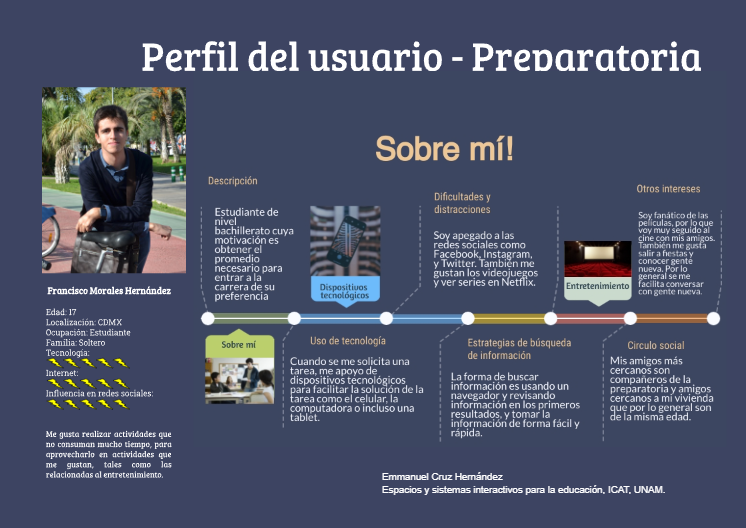
\includegraphics[width=0.60\textwidth]{Cap4/Figuras/Prepa.png}
  \caption{Modelo Persona de alumnos de bachillerato.}
  \label{fig:413}
\end{figure}

Por otro lado, se realizó un modelo Persona enfocado a estudiantes de primeros semestres de licenciatura. Este modelo es el resultado de la recopilación de datos de las actividades realizadas con los alumnos de primeros semestres de la facultad de ciencias.

En el modelo Persona de la Figura \ref{fig:414} se presenta a Abraham, un estudiante de licenciatura de 20 años, con agilidad para manejar diferentes herramientas en Internet, pero a diferencia de Francisco, por el consumo de tiempo de su carrera, no tiene mucha influencia en las redes sociales. Abraham se siente atraído e interesado por conocer nuevos lugares y aprender nuevas cosas con el fin de crecer en el ámbito académico y profesional.

Abraham se siente motivado por terminar su carrera, obtener su título y encontrar un trabajo que le agrade y que cuente con un ambiente en el que se sienta cómodo. Durante su tiempo libre, trata de aprender sobre diferentes temas relacionados al arte, tal como pintura, música o lectura.

Cuando Abraham realiza una investigación, se apoya de diferentes fuentes de información, entre las cuales se encuentran los libros, revistas científicas, bibliotecas virtuales y blogs en la web. Siempre procura obtener la información más confiable y clara, que le permita entender de forma sencilla los temas que busca.

Abraham suele utilizar algunas aplicaciones que le permitan tener un hábito de productividad. Entre las aplicaciones que usa para organizar su tiempo de forma flexible, se encuentran Trello, Slack y Asana.

Algunos intereses de Abraham son las series de género dramático y suspenso. Por lo general utiliza la plataforma Netflix.

\begin{figure}[H]
% \begin{figure}
  \centering
  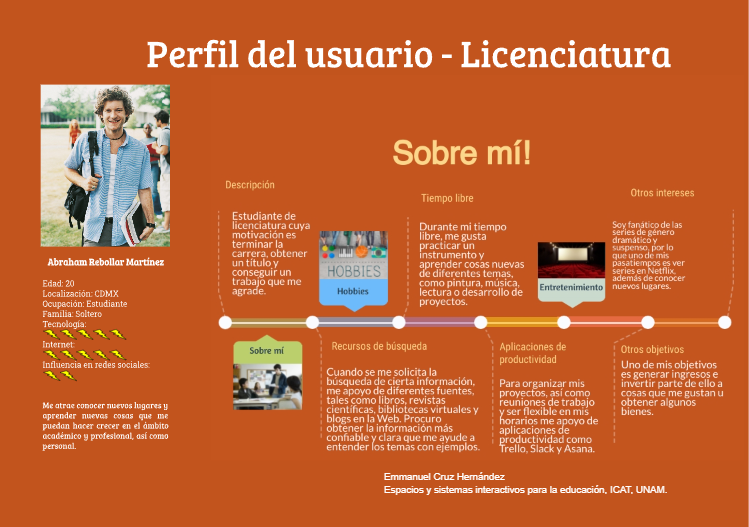
\includegraphics[width=0.60\textwidth]{Cap4/Figuras/Lic.png}
  \caption{Modelo Persona de alumnos de primeros semestres de licenciatura.}
  \label{fig:414}
\end{figure}

%------------------------------------------------------------
%	Diseño de Customer Journey Map para la skill
%------------------------------------------------------------

\subsection{Diseño de Customer Journey Map para la skill}
\label{DisenioCustomerJourneyMapSkillcapIV}

Con el fin de facilitar la comprensión de cómo se comportan los usuarios de forma general en diferentes contextos, se realizó un Customer Journey Map, que muestra los puntos generales que realizan los alumnos para completar una actividad.

En cada punto del proceso de investigación de información, se analizan sus acciones, objetivos, pensamientos, emociones y oportunidades. En la Figura \ref{fig:415} se muestra el flujo representado por un Customer Journey Map.

\begin{figure}[H]
% \begin{figure}
  \centering
  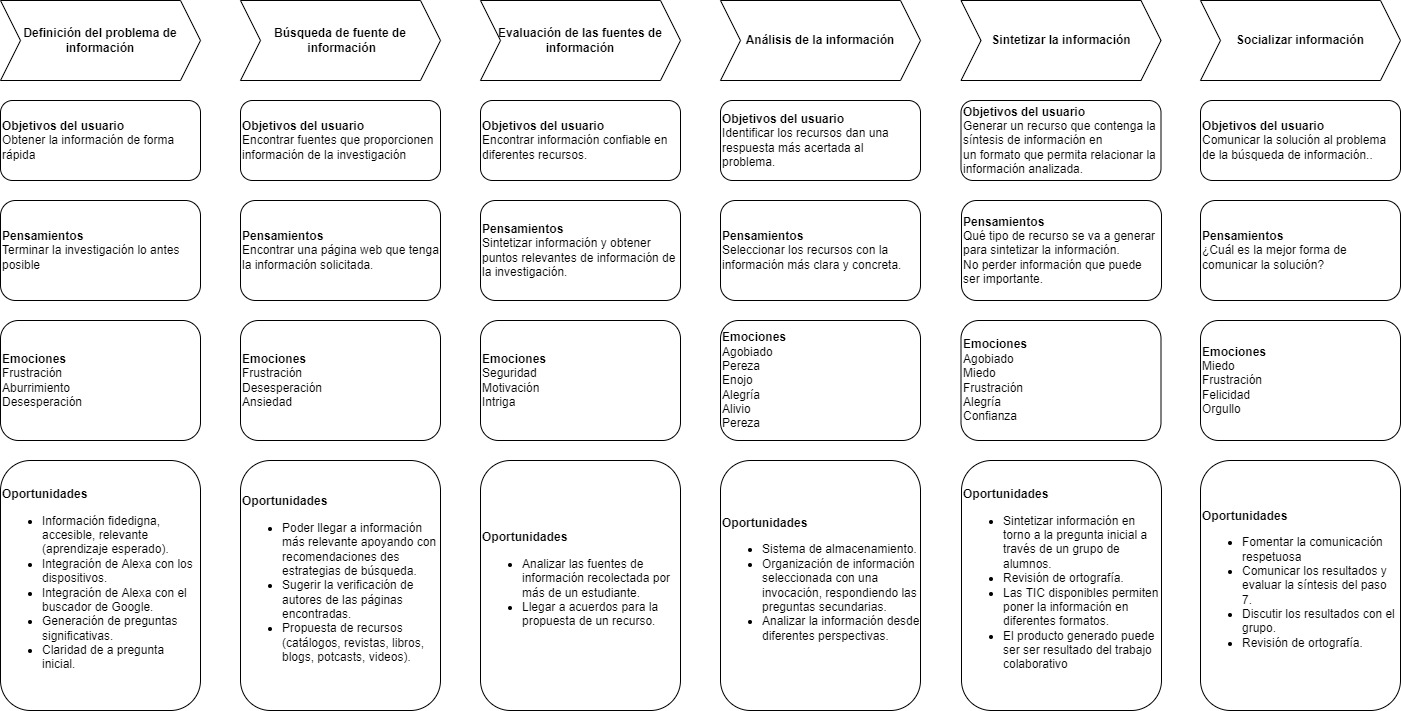
\includegraphics[width=0.80\textwidth]{Cap4/Figuras/Customer Journey Map Skill.jpg}
  \caption{Customer Journey Map del proceso de búsqueda de información de los alumnos.}
  \label{fig:415}
\end{figure}

El Customer Journey Map se divide en seis pasos o fases principales:

\begin{enumerate}
  \item Definición del problema de información.
  \item Búsqueda de fuente de información.
  \item Evaluación de las fuentes de información.
  \item Análisis de la información.
  \item Sintetizar la información.
  \item Socializar información.
\end{enumerate}

%------------------------------------------------------------
%	Adaptación del Modelo Gavilán
%------------------------------------------------------------

\subsection{Adaptación del Modelo Gavilán}
\label{AdaptacionModeloGavilancapIV}

A partir de la información obtenida en cada una de las etapas del Customer Journey Map, se obtuvieron oportunidades a considerar para el diseño de la skill, las cuales están enfocadas al entorno de la consola de desarrollo de Alexa. En cada etapa se obtuvieron las siguientes oportunidades.

\begin{itemize}
  \item Definición del problema de información
  \begin{itemize}
    \item Apoyar con la generación de una pregunta inicial y preguntas secundarias.
  \end{itemize}
  \item Búsqueda de fuente de información
  \begin{itemize}
    \item Dar prioridad a las fuentes de información provenientes de una institución educativa.
  \end{itemize}
  \item Evaluación de las fuentes de información
  \begin{itemize}
    \item Permitir al usuario elegir la fuente de información donde investigar.
  \end{itemize}
  \item Análisis de la información
  \begin{itemize}
    \item Almacenar información seleccionada en una estructura de datos por medio de una invocación de la skill.
  \end{itemize}
  \item Sintetizar la información
  \begin{itemize}
    \item Diseñar un mecanismo para recordar el nombre de la tarea, las fuentes consultadas y la fecha de entrega.
  \end{itemize}
  \item Socializar información
  \begin{itemize}
    \item Decir la información final de la investigación recopilada con la skill.
    \item Sugerir estrategias para compartir la información (modelos para comunicar la información).
  \end{itemize}
\end{itemize}

A partir de los puntos anteriores, se diseñó una adaptación en la que el Modelo Gavilán se puede acoplar de la forma más satisfactoria para cubrir las oportunidades enfocadas al desarrollo de la skill. Cabe mencionar que el Modelo Gavilán es un modelo que define sus pasos como guía para seguir un proceso de investigación de información, sin embargo, este puede ser adaptado a las necesidades del problema para ser aplicado de la forma más conveniente.

La adaptación del Modelo Gavilán se conforma a partir de los siguientes pasos, subpasos y objetivos:

\begin{enumerate}
  \item \textbf{Definición del problema de investigación.}
  \begin{enumerate}[1.]
    \item \textbf{Sugerir una pregunta inicial y analizarla.} La skill podrá crear un listado de sugerencias de preguntas relacionadas al tema de la investigación. En esta etapa el usuario podrá comenzar la investigación con la pregunta inicial que le parezca más adecuada a sus objetivos.
    \item \textbf{Elegir la construcción de un plan de investigación.} A partir de la selección de una pregunta, el usuario comienza a crear un plan de construcción con la limitación de un tema general en un subtema.
    \item \textbf{Sugerir preguntas secundarias.} Las preguntas sugeridas por la skill, que no fueron elegidas como pregunta inicial, fungen como preguntas secundarias, que abordan subtemas alternos al principal.
  \end{enumerate}
  \item \textbf{Búsqueda y evaluación de fuentes de información.}
  \begin{enumerate}[1.]
    \item \textbf{Identificar y seleccionar las fuentes de información más adecuadas.} La skill tendrá la capacidad de sugerir diferentes fuentes de información de distintas páginas en la web. Antes de extraer información, proporciona las fuentes de información para que el usuario analice y determine cuáles son las más adecuadas para la investigación.
    \item \textbf{Acceder a las fuentes de información seleccionadas.} Una vez elegida una fuente de información, la skill podrá proporcionar información específica sobre el contenido de la fuente.
    \item \textbf{Evaluar las fuentes de información encontradas.} El usuario podrá escuchar por medio de la skill, la información para poder analizarla y determinar si el contenido es útil para la investigación final.
  \end{enumerate}
  \item \textbf{Análisis de la información.}
  \begin{enumerate}[1.]
    \item \textbf{Elegir la información más adecuada para responder las preguntas secundarias.} El usuario podrá recolectar información que permita responder de manera directa a puntos específicos de un tema o subtema. La skill proporcionará un mecanismo de almacenamiento de fragmentos de información que responde a preguntas secundarias.
    \item \textbf{Leer, entender, comparar y evaluar la información seleccionada para responder las preguntas secundarias.} La información recopilada podrá ser consultada en cualquier momento desde la skill, con el fin de comparar y evaluar el contenido de la investigación.
  \end{enumerate}
  \item \textbf{Síntesis y socialización de la información.}
  \begin{enumerate}[1.]
    \item \textbf{Responder la pregunta inicial.} Cuando se termina el proceso de investigación con el apoyo de la skill, ésta enviará las fuentes de información a un dispositivo móvil, que en conjunto responderá a la pregunta inicial.
    \item \textbf{Elaborar un producto concreto y comunicar los resultados de la investigación.} La skill proporciona un mecanismo para seguir una estrategia de búsqueda de información, sin embargo, no elabora un producto final. La skill podrá sugerir diferentes modelos y estrategias para representar la información consultada.
  \end{enumerate}
\end{enumerate}

%------------------------------------------------------------
%	Diseño de la skill
%------------------------------------------------------------

\section{Diseño de la skill}
\label{DisenioSkillcapIV}

A partir de los resultados obtenidos con las herramientas creadas en la etapa del análisis del usuario y la adaptación del Modelo Gavilán, se crearon herramientas para facilitar el diseño de la skill.

La primera herramienta de apoyo para conocer la interacción de la skill con un usuario, considerando la adaptación del Modelo Gavilán, fue una recopilación de imágenes que forman un Storyboard.

Posteriormente, se diseñó un esquema para definir la navegación de la skill. Esta herramienta considera el flujo de la forma de interacción de un usuario con la skill mostrado en el Storyboard.

%------------------------------------------------------------
%	Storyboard
%------------------------------------------------------------

\subsection{Storyboard}
\label{StoryboardcapIV}

% REFERENCIA
La fundación de interacción de diseño (2022c) señala que es posible crear un guión gráfico con cada uno de los pasos de un proceso. Cada una de las imágenes muestra el proceso de alguna actividad para tener una mejor visión de cómo un usuario puede interactuar con un producto o servicio, a este conjunto de imágenes se conoce como storyboard.

Antes de comenzar con la implementación, se creó un storyboard para visualizar de una forma más clara la forma de interacción, así como los diálogos posibles y las respuestas que podría devolver la skill. A continuación se presentan los cuadros del storyboard de cada uno de los pasos definidos en el Customer Journey Map de la sección \ref{DisenioCustomerJourneyMapSkillcapIV}.

\begin{itemize}
  \item \textbf{Definición del problema de información.} El alumno se muestra frustrado por comenzar una investigación, en este caso, sobre la fotosíntesis. La skill provee un listado de preguntas sugeridas para seleccionar una pregunta inicial y comenzar con la investigación. Este proceso se puede visualizar en la Figura \ref{fig:416}.
  \begin{figure}[H]
  % \begin{figure}
    \centering
    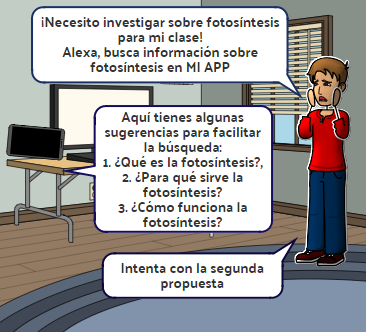
\includegraphics[width=0.40\textwidth]{Cap4/Figuras/01.png}
    \caption{Storyboard, definición del problema de información.}
    \label{fig:416}
  \end{figure}
  \item \textbf{Búsqueda de fuentes de información.} Durante la búsqueda de fuentes de información, se sugieren una serie de fuentes que contienen información relacionada a la pregunta inicial. El usuario analiza las fuentes de información y selecciona la que considera más adecuada. Este proceso se puede consultar en la Figura \ref{fig:417}.
  \begin{figure}[H]
  % \begin{figure}
    \centering
    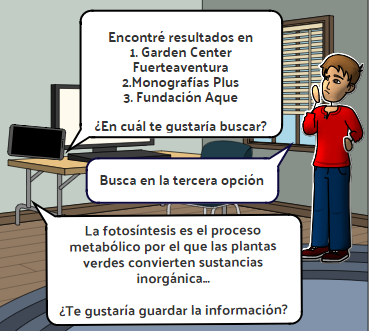
\includegraphics[width=0.40\textwidth]{Cap4/Figuras/02.png}
    \caption{Storyboard, búsqueda de fuentes de información.}
    \label{fig:417}
  \end{figure}
  \item \textbf{Evaluación de las fuentes de información.} Cuando se presenta la información extraída de la fuente seleccionada, el usuario analiza el contenido y determina si es útil para la investigación. En caso de ser útil, el usuario tiene la posibilidad de almacenar el fragmento de información. Este paso se puede visualizar en la Figura \ref{fig:418}.
  \begin{figure}[H]
    \centering
    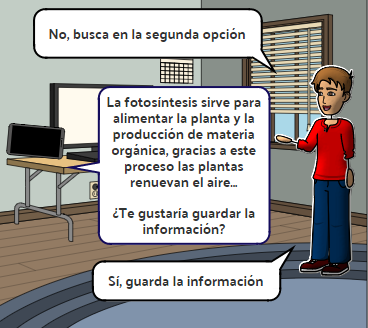
\includegraphics[width=0.40\textwidth]{Cap4/Figuras/03.png}
    \caption{Storyboard, evaluación de las fuentes de información.}
    \label{fig:418}
  \end{figure}
  \item \textbf{Análisis de la información.} El usuario analiza la información y determina si es necesario incluir más datos que sean útiles para la investigación final. El usuario interactúa con la skill de tal forma que puede consultar más contenido en otras fuentes de información y analizar el contenido hasta que considera que la información que ha obtenido es suficiente. Este paso se puede visualizar en la Figura \ref{fig:419}.
  \begin{figure}[H]
    \centering
    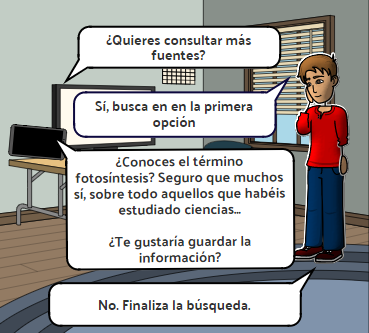
\includegraphics[width=0.40\textwidth]{Cap4/Figuras/04.png}
    \caption{Storyboard, análisis de la información.}
    \label{fig:419}
  \end{figure}
  \item \textbf{Sintetizar la información.} La skill provee una serie de recomendaciones para incluir durante la síntesis de la investigación, tal como las fuentes de información consultadas. Además, aporta un mecanismo de recordatorios para la entrega de una investigación. Este paso se puede visualizar en la Figura \ref{fig:420}.
  \begin{figure}[H]
    \centering
    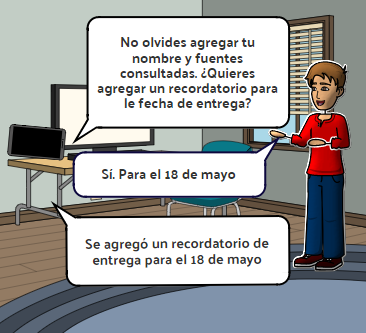
\includegraphics[width=0.40\textwidth]{Cap4/Figuras/05.png}
    \caption{Storyboard, sintetizar la información.}
    \label{fig:420}
  \end{figure}
  \item \textbf{Socializar información.} Finalmente, se dice toda la información recopilada durante el manejo de la skill. Además, la skill proporciona una serie de estrategias para compartir la información y se pueda elaborar un producto final. Este paso se puede visualizar en la Figura \ref{fig:421}.
  \begin{figure}[H]
    \centering
    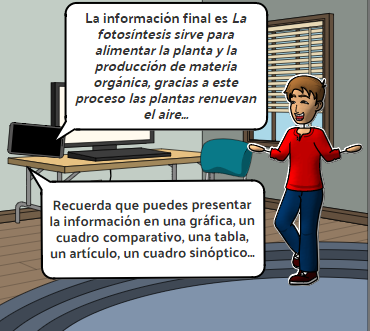
\includegraphics[width=0.40\textwidth]{Cap4/Figuras/06.png}
    \caption{Storyboard, socializar la información.}
    \label{fig:421}
  \end{figure}
\end{itemize}

%------------------------------------------------------------
%	Diagrama de navegación
%------------------------------------------------------------

\subsection{Diagrama de navegación}
\label{DiagramaNavegacioncapIV}

% REFERENCIA
La fundación de interacción de diseño (2022d) señala que un diagrama de flujo o de navegación, son diagramas que permiten visualizar de forma esquemática el flujo de un producto para resolver una tarea o subtarea.

El diagrama de navegación del Buscador Gavilán se divide en cinco secciones principales:

\begin{enumerate}
  \item \textbf{La selección de una pregunta inicial.} Se provee una sugerencia de pregunta inicial. El usuario tiene la opción de elegir o rechazar la pregunta sugerida.
  \begin{itemize}
    \item Si el usuario rechaza la pregunta sugerida, se presenta otra sugerencia y se repite este proceso.
    \item Si el usuario acepta la pregunta inicial sugerida, se pasa a la siguiente sección.
  \end{itemize}
  \item \textbf{La selección de una fuente de información.} La skill presenta una serie de fuentes de información para comenzar a extraer la información. Cada una de las sugerencias se van presentando una a una.
  \begin{itemize}
    \item Si el usuario rechaza la fuente de información sugerida, se presenta otra sugerencia y se repite este proceso.
    \item Si el usuario acepta la fuente de información sugerida, se pasa a la siguiente sección.
  \end{itemize}
  \item \textbf{Extracción, análisis y evaluación de la información.} La skill indaga en el contenido de la fuente de información, diciendo al usuario el contenido dividido en párrafos. Cuando se termina de leer un párrafo, la skill propone dos opciones para continuar el flujo.
  \begin{itemize}
    \item Si el usuario desea saber más contenido de la fuente, lee otro párrafo y realiza el mismo proceso de esta sección, además de tener la posibilidad de almacenar el contenido.
    \item Si el usuario prefiere seguir con el flujo, se da la posibilidad de indagar en más fuentes de información, regresando a la sección dos, o terminar con la investigación, pasando a la siguiente sección.
  \end{itemize}
  \item \textbf{Síntesis de la información.} La skill proporciona una serie de recomendaciones para incluir en el trabajo final, tal como el nombre y las fuentes de información. Además, da la posibilidad de agregar un recordatorio para la fecha de entrega. Si el usuario agrega u omite el recordatorio, ambos flujos pasan a la siguiente sección.
  \item \textbf{Socialización de la información.} En esta última sección se da un resumen del contenido extraído durante la búsqueda, así como el envío de las fuentes de información a la aplicación móvil de Alexa para indagar más en las fuentes originales.
\end{enumerate}

A continuación, se presenta el diagrama de navegación general de la skill en la Figura \ref{fig:422}, donde los diálogos en azul corresponden a la interacción del usuario, los diálogos en verde representan las respuestas de la skill y los apartados en blanco corresponde al inicio y término de ejecución de la skill.

\begin{figure}[H]
  \centering
  \includegraphics[width=0.90\textwidth]{Cap4/Figuras/DiagramaDeNavegación.png}
  \caption{Storyboard, socializar la información.}
  \label{fig:422}
\end{figure}

%------------------------------------------------------------
%	Implementación
%------------------------------------------------------------

\section{Implementación}
\label{ImplementacioncapIV}

Dado el análisis del problema, el análisis del usuario y las herramientas proporcionadas en la etapa de diseño, se implementó una skill llamada Buscador Gavilán, que tiene como objetivo abordar el problema encontrado en el análisis del problema. El logo de la skill se presenta en la Figura \ref{fig:423}.

\begin{figure}[H]
  \centering
  
\includegraphics[width=0.40\textwidth]{Cap4/Figuras/LogoSkill.png}
  \caption{Logo del Buscador Gavilán.}
  \label{fig:423}
\end{figure}

La skill funge como un apoyo para la búsqueda de información, en la que se guía a un usuario a realizar una búsqueda, basada en la adaptación de los cuatro pasos definidos en el Modelo Gavilán: definición del problema de información, búsqueda de fuente de información, evaluación de las fuentes de información y análisis de la información.

A partir de las herramientas construidas en la etapa de análisis del usuario, se crearon herramientas para el diseño de la skill. En particular, el diseño de la skill se basa en el diagrama de navegación para la construcción del flujo de interacción con el usuario.

%------------------------------------------------------------
%	Invocaciones del Buscador Gavilán
%------------------------------------------------------------

\subsection{Invocaciones del Buscador Gavilán}
\label{InvocacionesBuscadorGavilancapIV}

El Buscador Gavilán es una skill que entra en la categoría de skills personalizadas, por lo que requiere un nombre de invocación. El comando de invocación de una skill es la forma en que se solicita la llamada de la misma para comenzar a ejecutar su funcionamiento.

La skill Buscador Gavilán reconoce dos tipos de invocaciones: invocaciones sin solicitud e invocación solicitada sólo por nombre, tal como se muestra en los siguientes ejemplos:

\begin{itemize}
  \item Alexa, abre Buscador Gavilán - invocación sin solicitud
  \item Alexa, comienza Buscador Gavilán - invocación sin solicitud
  \item Alexa, Buscador Gavilán - invocación solicitada sólo por nombre
\end{itemize}

Es importante mencionar que el nombre de invocación de la skill siempre va seguido de la palabra de activación “Alexa”. Dependiendo de la configuración del nombre de activación del dispositivo, este podría usar como palabras de activación “Echo” o “Amazon”.

Es importante mencionar que el nombre de invocación considera la entonación del usuario, por lo que el acento incorporado en el nombre de la skill es reconocido por los dispositivos con Alexa integrada.

%------------------------------------------------------------
%	Intenciones, declaraciones y slots del Buscador Gavilán
%------------------------------------------------------------

\subsection{Intenciones, declaraciones y slots del Buscador Gavilán}
\label{IntencionesDeclaracionesSlotscapIV}

Las intenciones de la skill cuentan con conjunto de declaraciones cada una. A su vez, algunas declaraciones cuentan con uno o más slots. Cada intención de la skill está diseñada para resolver una subtarea específica del problema general en cada proceso de la búsqueda de información con el Buscador Gavilán. A continuación se presentan las intenciones reconocidas por la skill y la subtarea que resuelve, así como las declaraciones y slots utilizados.

%------------------------------------------------------------
%	AMAZON.CancelIntent
%------------------------------------------------------------

\subsubsection{AMAZON.CancelIntent}
\label{CancelIntentcapIV}

Esta intención se encuentra predefinida por la consola de desarrollo de Alexa como una intención requerida, por lo que no puede ser eliminada. Su objetivo es englobar todas las declaraciones para terminar la ejecución de una subtarea, sin salir de la skill.

Al ser una intención que está definida por omisión, las declaraciones se encuentran predefinidas con la misma. Entre las declaraciones posibles para invocar la intención se encuentran las siguientes palabras y frases:

\begin{itemize}
  \item Cancelar
  \item Cancela
\end{itemize}

%------------------------------------------------------------
%	AMAZON.HelpIntent
%------------------------------------------------------------

\subsubsection{AMAZON.HelpIntent}
\label{HelpIntentcapIV}

Esta intención se encuentra predefinida por la consola de desarrollo de Alexa como una intención requerida, por lo que no puede ser eliminada. Está enfocada a englobar las declaraciones que sirven como guía al usuario, brindando instrucciones de ayuda para poder utilizar la skill.

Entre las declaraciones posibles para invocar la intención se encuentran las siguientes:

\begin{itemize}
  \item Ayuda
  \item Quiero ayuda
\end{itemize}

%------------------------------------------------------------
%	AMAZON.StopIntent
%------------------------------------------------------------

\subsubsection{AMAZON.StopIntent}
\label{StopIntentcapIV}

Esta intención se encuentra predefinida por la consola de desarrollo de Alexa como una intención requerida, por lo que no puede ser eliminada. A diferencia de la intención AMAZON.CancelIntent, esta intención engloba las declaraciones para terminar la ejecución completa de la skill.

Entre las declaraciones posibles para invocar la intención se encuentran las siguientes palabras y frases:

\begin{itemize}
  \item Para
  \item Termina
  \item Cierra skill
  \item Cierra la skill
\end{itemize}

%------------------------------------------------------------
%	AMAZON.NavigateHomeIntent
%------------------------------------------------------------

\subsubsection{AMAZON.NavigateHomeIntent}
\label{NavigateHomeIntentcapIV}

Esta intención se encuentra predefinida por la consola de desarrollo de Alexa como una intención requerida, por lo que no puede ser eliminada, sin embargo, esta intención está configurada para funcionar únicamente con dispositivos que cuentan con pantalla.

Su función es cerrar la skill y posicionar la vista de la pantalla en la pantalla de inicio de Alexa. La intención puede ser invocada por medio de las siguientes declaraciones:

\begin{itemize}
  \item Ve al inicio
  \item Inicio
\end{itemize}

%------------------------------------------------------------
%	AMAZON.FallbackIntent
%------------------------------------------------------------

\subsubsection{AMAZON.FallbackIntent}
\label{FallbackIntentcapIV}

Esta intención se encuentra predefinida por la consola de desarrollo de Alexa como una intención requerida, por lo que no puede ser eliminada. Su función es englobar las declaraciones que dan orientación al usuario cuando alguna solicitud no fue reconocida por las declaraciones válidas de cualquier intención.

Esta intención no cuenta con declaraciones predefinidas, ya que se invoca únicamente en caso de no reconocer la solicitud con alguna declaración válida.

%------------------------------------------------------------
%	tellTopicIntent
%------------------------------------------------------------

\subsubsection{tellTopicIntent}
\label{tellTopicIntentcapIV}

Es una intención personalizada que tiene como objetivo englobar las declaraciones que obtienen el tema general de la investigación. Esta intención es el comienzo del flujo de interacción con la skill, en donde es necesario conocer el tema del cual se buscará información.

Dada la gran variedad de formas en que se puede solicitar información de un tema, se crearon sesenta y siete declaraciones, entre las que se encuentran las siguientes:

\begin{itemize}
  \item dime sobre el tema de \{searchWord\}
  \item dame el tema \{searchWord\}
  \item quiero saber sobre el tema de \{searchWord\}
  \item quiero saber sobre el tema \{searchWord\}
  \item sobre el tema \{searchWord\}
  \item por qué \{searchWord\}
  \item donde puedo \{searchWord\}
  \item donde fue la \{searchWord\}
  \item cuando fue el \{searchWord\}
  \item cómo funciona la \{searchWord\}
  \item que es el \{searchWord\}
  \item debo investigar acerca de \{searchWord\}
  \item dime de \{searchWord\}
  \item busca sobre \{searchWord\}
\end{itemize}

Cada una de las declaraciones definidas anteriormente cuenta con un slot, llamado \textit{searchWord}. Este slot es la variable que almacena en texto el tema con el que se comenzará la investigación.

El slot \textit{searchWord} es de tipo AMAZON.SearchQuery, el cual convierte la información en una palabra o frase que puede ser ingresada en un motor de búsqueda estándar. Dado que la búsqueda de información se basa en la web, este tipo de slot es el más adecuado para obtener la información acerca del tema general de la investigación.

%------------------------------------------------------------
%	AMAZON.YesIntent
%------------------------------------------------------------

\subsubsection{AMAZON.YesIntent}
\label{YesIntentcapIV}

Esta intención se encuentra predefinida por la consola de desarrollo de Alexa como una intención no requerida u opcional. Su función es englobar todas las declaraciones para reconocer aquellas entradas que pueden ser consideradas como una afirmación. En la skill, se utiliza para reconocer declaraciones que confirman una pregunta inicial o una fuente de información a investigar.

Dado que la intención es predefinida, algunas declaraciones ya se encuentran incorporadas por omisión,tales como las siguientes:

\begin{itemize}
  \item Sí
  \item Confirmo
  \item Afirmativo
  \item Así es
  \item Es correcto
\end{itemize}

A su vez, se incorporaron otras declaraciones acordes a la skill para ser reconocidas con el mismo propósito de las declaraciones ya existentes. Entre estas declaraciones personalizadas se encuentran las siguientes:

\begin{itemize}
  \item usa esa sugerencia
  \item quiero esa recomendación
  \item elige la referencia
  \item consulta la referencia
  \item utiliza la pregunta
  \item consulta esa referencia
  \item quiero comenzar por esa opción
  \item sí es la opción
\end{itemize}

%------------------------------------------------------------
%	AMAZON.NoIntent
%------------------------------------------------------------

\subsubsection{AMAZON.NoIntent}
\label{NoIntentcapIV}

Esta intención se encuentra predefinida por la consola de desarrollo de Alexa como una intención no requerida u opcional. Su función es englobar todas las declaraciones para reconocer aquellas entradas que pueden ser consideradas como una negación. En la skill, esta intención es utilizada para reconocer declaraciones para sugerir una pregunta inicial al rechazar una propuesta, o dar una sugerencia de una fuente de información al ser rechazada una propuesta.

Dado que la intención es predefinida, algunas declaraciones ya se encuentran incorporadas por omisión, entre las que se encuentran las siguientes:

\begin{itemize}
  \item No
  \item Estoy en desacuerdo
  \item No es
  \item Negativo
\end{itemize}

Al igual que la intención AMAZON.YesIntent, se incorporaron otras declaraciones acordes a la skill para ser reconocidas con el mismo propósito de las declaraciones ya existentes. Entre estas declaraciones personalizadas se encuentran las siguientes:

\begin{itemize}
  \item sugiere otra pregunta inicial
  \item dame otra pregunta
  \item dame más recomendaciones
  \item dame más sugerencias
  \item busca otra recomendación
  \item busca más
  \item recomiendame otra referencia
  \item consulta más fuentes
  \item busca otra opción
  \item siguiente opción
  \item intenta con otra
\end{itemize}

%------------------------------------------------------------
%	nextInfoIntent
%------------------------------------------------------------

\subsubsection{nextInfoIntent}
\label{nextInfoIntentcapIV}

Es una intención personalizada que tiene el propósito de englobar todas las declaraciones enfocadas a obtener más información de un recurso. Cuando un usuario indaga en el contenido de una fuente de información, esta se presenta por párrafos. Las declaraciones englobadas en ésta intención están enfocadas a obtener el contenido del párrafo siguiente del actual, dentro de la fuente de información elegida.

Las declaraciones definidas para esta intención son las siguientes:

\begin{itemize}
  \item dime más sobre el tema
  \item dime más
  \item quiero más información
  \item dame más información
  \item más información
  \item dime el siguiente
  \item lee siguiente
  \item lee el siguiente párrafo
  \item extiende la información
  \item quiero saber más
  \item siguiente párrafo
\end{itemize}

%------------------------------------------------------------
%	continueIntent
%------------------------------------------------------------

\subsubsection{continueIntent}
\label{continueIntentcapIV}

Es una intención personalizada que tiene el propósito de englobar todas las declaraciones enfocadas a dar la posibilidad de terminar la investigación del contenido de la fuente actual.

Entre las declaraciones definidas en esta intención se encuentran las siguientes:

\begin{itemize}
  \item ir al siguiente paso de la investigación
  \item ir al siguiente paso
  \item sigue la investigación
  \item continuar con la investigación
\end{itemize}

%------------------------------------------------------------
%	endInvestigationIntent
%------------------------------------------------------------

\subsubsection{endInvestigationIntent}
\label{endInvestigationIntentcapIV}

Es una intención personalizada que tiene el propósito de englobar todas las declaraciones enfocadas a terminar la etapa de búsqueda de información, por lo que termina de recomendar fuentes de información y leer contenido de las mismas.

Entre las declaraciones definidas para invocar esta intención se encuentran las siguientes:

\begin{itemize}
  \item concluye la investigación
  \item finaliza la investigación
  \item termina la investigación
\end{itemize}

%------------------------------------------------------------
%	addReminderIntent
%------------------------------------------------------------

\subsubsection{addReminderIntent}
\label{addReminderIntentcapIV}

Es una intención personalizada que tiene el propósito de englobar todas las declaraciones que permiten agregar un recordatorio dentro del sistema de la skill.

Algunas declaraciones definidas para esta intención son las siguientes:

\begin{itemize}
  \item agrega el recordatorio para el día \{date\}
  \item crea el recordatorio para el día \{date\}
  \item agrega el recordatorio para el \{date\}
  \item agrega un recordatorio el \{date\}
\end{itemize}

En las declaraciones definidas, se utiliza un slot llamado date. Este slot es de tipo AMAZON.DATE, el cual transforma las entradas a fechas en el formato 2022-09-00T9. La creación de un recordatorio en la lista de recordatorios del servicio de Alexa, requiere de un día y un mes de forma obligatoria, por lo que el tipo AMAZON.DATE es el más adecuado para almacenar esta información, ya que contiene la información requerida.

En el conjunto de declaraciones de esta intención, existen declaraciones que no contienen el dato de la fecha como un slot, tales como los siguientes:

\begin{itemize}
  \item crea recordatorio
  \item agrega recordatorio
\end{itemize}

El slot llamado \textit{date}, está configurado como un slot obligatorio. Cuando alguna de las declaraciones que no contienen el slot es conocido, la intención realiza solicitudes extra para obtener la fecha. Algunas de las solicitudes realizadas por esta intención son las siguientes.

\begin{itemize}
  \item Dime la fecha de entrega de tu tarea
  \item Dime la fecha en que te recordaré la entrega
  \item ¿Cuándo te lo recuerdo?
  \item ¿Qué día quieres que te recuerde la entrega?
\end{itemize}

Las respuestas válidas a estas solicitudes son las siguientes:

\begin{itemize}
  \item para el \{date\}
  \item para \{date\}
  \item crea un recordatorio para \{date\}
  \item agrega recordatorio para \{date\}
  \item agrega el recordatorio el \{date\}
\end{itemize}

En estas solicitudes se pide el dato \textit{date} obligatoriamente para poder invocar correctamente esta intención.

%------------------------------------------------------------
%	omitIntent
%------------------------------------------------------------

\subsubsection{omitIntent}
\label{omitIntentcapIV}

Es una intención personalizada que tiene el propósito de englobar todas las declaraciones que omiten la declaración de un recordatorio. Dado que los recordatorios fungen como una funcionalidad no obligatoria, es posible saltarlos cuando se reconoce alguna de las declaraciones definidas para esta intención. Entre las que se encuentran las siguientes declaraciones:

\begin{itemize}
  \item omitir recordatorio
  \item omite recordatorio
\end{itemize}

%------------------------------------------------------------
%	lastRequestIntent
%------------------------------------------------------------

\subsubsection{lastRequestIntent}
\label{lastRequestIntentcapIV}

Es una intención personalizada que tiene el propósito de englobar todas las declaraciones que permiten recordar la última solicitud realizada por un usuario. Entre las declaraciones de esta intención se encuentran las siguientes:

\begin{itemize}
  \item Recuérdame la última solicitud
  \item Cuál fue la última solicitud
  \item Dime la última solicitud
  \item Recuérdame la última petición
  \item Recuérdame donde estaba
\end{itemize}

%------------------------------------------------------------
%	Custom Search JSON API
%------------------------------------------------------------

\subsection{Custom Search JSON API}
\label{CustomSearchJSONAPIcapIV}

% REFERENCIA
Google Developers (2022) señala que el API JSON de búsqueda personalizada es un API que permite desarrollar sitios o aplicaciones para buscar y mostrar resultados dados por un motor de búsqueda.

Esta API permite recibir una frase en texto para comenzar la búsqueda. Los resultados encontrados en el motor de búsqueda se devuelven en formato JSON, del cual se puede extraer información de cada resultado, tal como su URL, descripción, dominio, título, lenguaje, entre otros.

Google Developers ofrece el servicio llamado \textit{Custom Search JSON API} con el control de un API Key, que permite identificar un cliente en Google, ya que el API Key está asociada a una cuenta de correo electrónico de Gmail.

A su vez, el API key controla ciertas configuraciones sobre la búsqueda que pueden definirse desde la consola de desarrollo de Google Developers. Algunas de estas configuraciones son restricciones de clave, restricciones de aplicaciones, restricciones de sitios web y restricciones de API.

La construcción básica para obtener los servicios del API JSON de búsqueda personalizada en Python se define de la siguiente forma:

\begin{tcolorbox}[colback=white!25!white,colframe=blue]
  \begin{minted}{python}
from apiclient.discovery import build

api_key = 'API-KEY'
resource = build("customsearch", 'v1', developerKey=api_key).cse()
  \end{minted}
\end{tcolorbox}

Donde API-KEY es la credencial generada por la consola de desarrollo de Google Developers para hacer uso del servicio.

El objeto \textit{resource}, construido en el código anterior, cuenta con un método llamado \textit{list}, el cual permite listar todos los resultados de una página que se mostrarían en un motor de búsqueda convencional como Google, Firefox, Safari, entre otros. La estructura básica para la obtención de resultados desde la API en Python, se muestra a continuación.

\begin{tcolorbox}[colback=white!25!white,colframe=blue]
  \begin{minted}{python}
results = resource.list(q=topic, cx='7931d2f657f7b38a2').execute()
  \end{minted}
\end{tcolorbox}

Donde:

\begin{itemize}
  \item \textbf{q:} corresponde a una palabra o frase que será el tema del que se buscarán resultados en el motor de búsqueda.
  \item \textbf{cx:} corresponde al ID del motor de búsqueda que se usará para realizar la solicitud.
  \item \textbf{results:} es un objeto tipo JSON con la respuesta obtenida de la solicitud. En este objeto se almacenan los resultados encontrados en el motor de búsqueda.
\end{itemize}

%------------------------------------------------------------
%	Generación de preguntas y búsqueda de fuentes
%------------------------------------------------------------

\subsubsection{Generación de preguntas y búsqueda de fuentes}
\label{GeneracionPreguntasBusquedaFuentescapIV}

La generación de preguntas de sugerencia de la skill se apoya del API JSON de búsqueda personalizada para generar sugerencias de preguntas. La forma en que se generan es a partir de la búsqueda de la concatenación de un tema general y las principales palabras que conforman una pregunta, tales como qué, cómo, entre otras.

Cada una de las sugerencias encontradas es filtrada para extraer sólo aquellas apariciones de preguntas, tal como se muestra a continuación.

\begin{tcolorbox}[colback=white!25!white,colframe=blue]
  \begin{minted}{python}
whyQuestion = resource.list(q='por que '+topic,cx='7931d2f657f7b38a2').execute()
whatQuestion = resource.list(q='que '+topic,cx='7931d2f657f7b38a2').execute()
whenQuestion = resource.list(q='cuando '+topic, cx='7931d2f657f7b38a2').execute()
whoQuestion = resource.list(q='quien '+topic, cx='7931d2f657f7b38a2').execute()
howQuestion = resource.list(q='como '+topic, cx='7931d2f657f7b38a2').execute()
  \end{minted}
\end{tcolorbox}

Las variables \textit{whyQuestion}, \textit{whatQuestion}, \textit{whenQuestion}, \textit{whoQuestion} y \textit{howQuestion} contienen una respuesta a los resultados encontrados en el motor de búsqueda, que posteriormente son filtrados por título, donde se verifica que existe un signo de interrogación, el cual denota una pregunta.

Cuando una pregunta es seleccionada como pregunta inicial, se aprovecha el funcionamiento del servicio de búsqueda personalizada para obtener resultados asociados a una pregunta, tal como sigue en el siguiente fragmento de código.

\begin{tcolorbox}[colback=white!25!white,colframe=blue]
  \begin{minted}{python}
resources = resource.list(q=selectedQuestion, cx='7931d2f657f7b38a2').execute()
  \end{minted}
\end{tcolorbox}

Donde:

\begin{itemize}
  \item \textbf{selectedQuestion:} corresponde a una pregunta seleccionada del conjunto de preguntas sugeridas.
  \item \textbf{resources:} contiene los resultados de la búsqueda que fungen como fuentes de información para la skill.
\end{itemize}

%------------------------------------------------------------
%	Web Scraping
%------------------------------------------------------------

\subsection{Web Scraping}
\label{WebScrapingcapIV}

% REFERENCIA
De acuerdo con Bo (2017), el Web Scraping es una técnica para extraer datos de la World Wide Web (www). La información que se puede extraer de la web con la técnica de Web Scraping puede ir desde texto, hasta imágenes y videos. A su vez, permite recopilar grandes cantidades de datos bien organizados en diferentes escenarios que van desde extracciones asistidas por humanos hasta su aplicación en sistemas completamente automatizados.

% REFERENCIA
Bo (2017) señala que el Web Scraping se puede dividir en dos pasos secuenciales: adquirir los recursos web y extraer la información de los datos adquiridos. La técnica para llevar a cabo el primer paso, requiere de una solicitud de tipo HTTP, la cual se forma por una solicitud GET con la URL de la dirección web donde se extraerán los datos. Posteriormente, el proceso de extracción analiza, formatea y organiza los datos en un formato estructurado dentro un objeto de tipo JSON.

Cabe mencionar que aunque el Web Scraping es una técnica poderosa para recopilar grandes cantidades de datos, es importante configurar y programar su funcionamiento de forma ética y responsable. Es decir, la extracción de datos debe considerar cuestiones legales, tales como los derechos de autor, los términos de servicios y el traspaso de bienes muebles, por lo que se vuelve relevante considerar un control responsable sobre el envío de solicitudes para la adquisición de datos, así como dar crédito a los autores. Algunos sitios web cuentan con mecanismos que previenen el ataque de sistemas malignos contra un servidor, por lo que es posible que la técnica de Web Scraping no pueda extraer información de dichos sitios web.

Para el presente proyecto, se implementó un web scraper con el fin de extraer la información de las fuentes de información encontradas en la web con la biblioteca BeautifulSoup, disponible para el lenguaje de programación Python.

En la clase WebScraper se implementan algunos métodos que facilitan el manejo de Web Scraping sobre un sitio web que contenga texto. Estos métodos se definen como se muestra en el siguiente código del anexo \ref{A1Anexo}.

%------------------------------------------------------------
%	Handlers
%------------------------------------------------------------

\subsection{Handlers}
\label{HandlerscapIV}

Los Handlers son funciones que implementan el comportamiento específico para una intención. Los Handlers permiten la construcción de la respuesta de una declaración asociada a la activación de una intención.

A continuación se presentan los Handlers implementados para el Buscador Gavilán y su función general.

\begin{itemize}
  \item \textbf{LaunchRequestHandler.} Implementa el handler con solicitud de tipo LaunchRequest, el cual se ejecuta una vez que se activa la skill. Este lanza un mensaje de bienvenida y una instrucción general de cómo comenzar una investigación con el Buscador Gavilán, tal como se muestra en el anexo \ref{A2Anexo}.
  \item \textbf{CancelOrStopIntentHandler.} Implementa el comportamiento definido para las intenciones AMAZON.CancelIntent y AMAZON.StopIntent, la cual lanza un mensaje de despedida al usuario antes de finalizar la ejecución de la skill, tal como se muestra en el anexo \ref{A3Anexo}.
  \item \textbf{HelpIntentHandler.} Implementa el comportamiento para la intención AMAZON.HelpIntent, la cual lanza una indicación de ayuda dependiendo del estado de la skill. Es decir, puede ayudar a iniciar una investigación, elegir alguna referencia, entre otros. Así mismo, regresa una frase con la última respuesta dada por la skill, tal como se muestra en el anexo \ref{A4Anexo}.
  \item \textbf{FallbackIntentHandler.} Implementa el comportamiento para la intención AMAZON.FallbackIntent, la cual se lanza cuando un comando no es reconocido por las declaraciones de las intenciones válidas. Lanza un mensaje para informar que la solicitud no fue entendida y se vuelva a repetir, así como comunicar la información de la última petición solicitada, tal como se muestra en el anexo \ref{A5Anexo}.
  \item \textbf{tellTopicIntentHandler.} Implementa el comportamiento de la intención tellTopicIntent. Este handler inicializa todos los valores al primer estado, ya que es la primera intención que se ejecuta al comenzar una nueva investigación en la skill. Por otra parte, se crea una nueva instancia de un scraper para comenzar con la generación de preguntas, las cuales se almacenan de forma global durante la ejecución de la skill. Lanza como respuesta una breve información sobre una pregunta inicial y la primera sugerencia de una pregunta, tal como se muestra en el anexo \ref{A6Anexo}.
  \item \textbf{yesAmazonIntentHandler.} Implementa el comportamiento de la intención AMAZON.YesIntent, la cual recibe una respuesta afirmativa. Este handler funciona para dos estados distintos de la skill: cuando se afirma una pregunta inicial y cuando se afirma una fuente de información. Cuando se afirma una pregunta inicial, se lee la pregunta elegida y se da la primera sugerencia de fuente de información relacionada a la pregunta. Cuando se afirma una fuente de información, se lee el autor del dominio del cual se extrae la información y se da conocimiento del primer párrafo de la fuente de información seleccionada, tal como se muestra en el anexo \ref{A7Anexo}.
  \item \textbf{noAmazonIntentHandler.} Implementa el comportamiento de la intención AMAZON.NoIntent, la cual recibe una declaración negativa. En los estados de la skill se puede negar una pregunta sugerida y una fuente de información, por lo que se divide en dos casos dependiendo del estado de la skill. Cuando se niega una pregunta sugerida, se lanza como respuesta otra pregunta sugerida, mientras que cuando se niega una fuente de información, se lanza como respuesta la siguiente fuente de información posible, tal como se muestra en el anexo \ref{A8Anexo}.
  \item \textbf{nextInfoIntentHandler.} Implementa la funcionalidad para la intención nextInfoIntent, la cual lanza como respuesta un párrafo de la fuente de información seleccionada en el proceso de selección de fuentes de información a partir de una pregunta inicial. En caso de no haber leído todos los párrafos, lanza un mensaje informativo para anunciar que no hay más contenido por dar como respuesta, tal como se muestra en el anexo \ref{A9Anexo}.
  \item \textbf{continueIntentHandler.} Implementa la funcionalidad de la intención continueIntent, la cual manda un mensaje informativo para elegir una de dos opciones: consultar más fuentes de información o terminar con el proceso de investigación, tal como se muestra en el anexo \ref{A10Anexo}.
  \item \textbf{endInvestigationIntentHandler.} Implementa la funcionalidad de la intención endInvestigationIntent, la cual da los datos informativos finales de la investigación, tal como consejos generales y una respuesta informativa para agregar u omitir recordatorios, tal como se muestra en el anexo \ref{A11Anexo}.
  \item \textbf{addReminderIntentHandler.} Implementa la funcionalidad para la intención addReminderIntent, la cual permite crear un recordatorio para la fecha de entrega de la investigación, tal como se muestra en el anexo \ref{A12Anexo}.
  \item \textbf{omitIntentHandler.} Implementa la funcionalidad para la intención omitIntent, la cual permite saltar la programación de un recordatorio, dando un resumen sobre la información recopilada durante la investigación, así como dar consejos para crear un producto final con la información recuperada. Este handler finaliza la ejecución de la skill, tal como se muestra en el anexo \ref{A13Anexo}.
  \item \textbf{lastRequestIntentHandler.} Implementa la funcionalidad para la intención lastRequestIntent, la cual permite al usuario saber cuál fue la respuesta de la última solicitud hecha en la skill. Lanza como respuesta la última oración dada por la skill, tal como se muestra en el anexo \ref{A14Anexo}.
\end{itemize}

%------------------------------------------------------------
%	Evaluación de la skill
%------------------------------------------------------------

\section{Evaluación de la skill}
\label{EvaluacionSkillcapIV}

La evaluación es una de las etapas del proceso iterativo del diseño centrado en el usuario, el cual consiste en realizar una serie de pruebas con distintas herramientas, con el fin de identificar los posibles problemas durante el manejo de un producto. Por otra parte, se logran identificar procedimientos, limitaciones y problemas en el diseño. En este apartado se detallan las herramientas usadas para aplicar la evaluación a la skill Buscador Gavilán, así como sus resultados.

%------------------------------------------------------------
%	Herramientas del proceso de evaluación de la skill y pruebas con usuarios
%------------------------------------------------------------

\subsection{Herramientas del proceso de evaluación de la skill y pruebas con usuarios}
\label{HerramientasEvaluacionPruebasUsuarioscapIV}

Para aplicar las pruebas, se toma como base el proceso de evaluación del grupo ESIE con cinco usuarios. Este proceso de evaluación se divide en tres fases principales: en la primera fase, un anfitrión o anfitriones dan la bienvenida a los usuarios y se obtiene información relevante sobre el usuario. A continuación se presentan las herramientas utilizadas en esta etapa:

\begin{itemize}
  \item \textbf{Cuestionario de entrada.} Tiene como propósito, conocer información relacionada a los intereses o tipos de dispositivos que usa el usuario. Esta información resulta útil para conocer la experiencia del usuario frente al funcionamiento de la skill. En el anexo \ref{B1Anexo} se muestra el cuestionario de entrada aplicado.
\end{itemize}

En la segunda fase, uno de los anfitriones lee un protocolo de bienvenida. Posteriormente, indica una serie de actividades que deben ser completadas por los usuarios. Mientras el usuario realiza las pruebas, un observador registra notas y resultados relevantes de cada actividad realizada por los usuarios.

\begin{itemize}
  \item \textbf{Protocolo de bienvenida.} El objetivo de este documento es presentar los objetivos de la evaluación, en este caso, evaluar la usabilidad de la skill Buscador Gavilán. En el anexo \ref{B2Anexo} se puede consultar el protocolo de bienvenida aplicado.
  \item \textbf{Actividades de la prueba.} Es una herramienta que define el listado de actividades que debe realizar un usuario. En el anexo \ref{B3Anexo} se presentan las actividades de la prueba aplicadas.
  \item \textbf{Guión de actividades para la evaluación.} Dada la dificultad para dar a conocer las actividades por voz a través de un anfitrión, las actividades se presentaron en un documento externo, donde se definen las actividades que puede realizar un usuario. En el anexo \ref{B4Anexo} se puede consultar el listado de actividades de la evaluación.
\end{itemize}

En la tercera y última fase de la evaluación, los usuarios responden algunos cuestionarios que permiten conocer la usabilidad y la experiencia al utilizar la skill.

\begin{itemize}
  \item \textbf{Cuestionario de usabilidad.} Este cuestionario contiene reactivos específicos para determinar la usabilidad de la skill Buscador Gavilán. El cuestionario de usabilidad aplicado se muestra en el anexo \ref{B5Anexo}.
  \item \textbf{Cuestionario de percepción subjetiva.} Este cuestionario ayuda a identificar particularidades de la interfaz respecto a la interfaz de usuario. El cuestionario de percepción subjetiva aplicado se muestra en el anexo \ref{B6Anexo}.
\end{itemize}

%------------------------------------------------------------
%	Evaluación con usuarios
%------------------------------------------------------------

\subsection{Evaluación con usuarios}
\label{EvaluacionUsuarioscapIV}

Con el fin de evaluar la usabilidad de la skill Buscador Gavilán de forma virtual, debido al confinamiento del COVID-19, se hicieron algunos ajustes a la aplicación del proceso de evaluación del grupo ESIE, además de ajustarlo para aplicarse a las características de una interfaz basada en reconocimiento por voz.

En el proceso de evaluación del grupo ESIE convencional, el moderador ordena una serie de actividades una a una. Para la evaluación de la skill, el moderador realizó una presentación con todas las funcionalidades posibles de la skill. Esta presentación ayudó a que los usuarios conocieran la interacción con la skill, con el fin de que el moderador no interviniera durante la interacción.

El segundo reto fue adaptar la forma de aplicar la evaluación a una modalidad virtual por medio de una reunión en la plataforma Zoom, en la que se encontraban conectados en línea al menos cuatro dispositivos, cada uno con una funcionalidad específica para poder llevar a cabo la evaluación.

\begin{enumerate}
  \item Un dispositivo con cámara activada para el moderador.
  \item Un dispositivo para el usuario.
  \item Un dispositivo que mostraba en cámara un dispositivo Echo Dot con la skill Buscador Gavilán instalada.
  \item Un dispositivo con cámara desactivada para el observador.
\end{enumerate}

En la Figura \ref{fig:424} se muestra una de las evaluaciones con los usuarios en las que se encuentran los cuatro dispositivos mencionados anteriormente.

\begin{figure}[H]
  \centering
  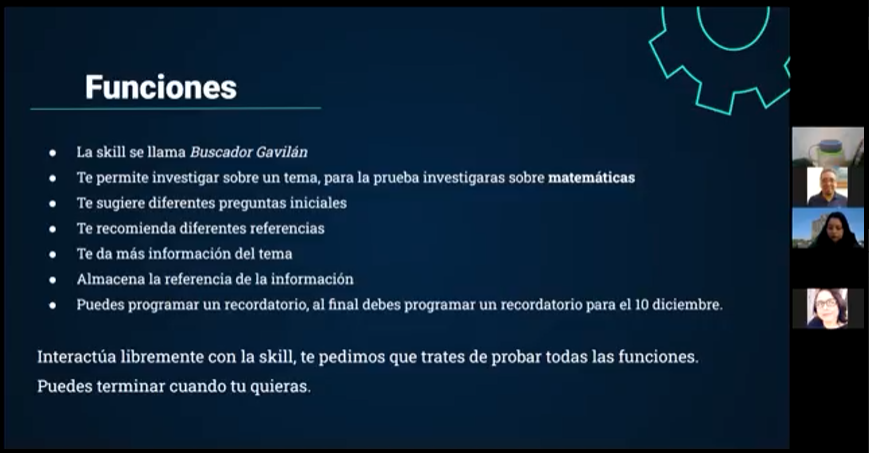
\includegraphics[width=0.70\textwidth]{Cap4/Figuras/Pruebas usuario 1.png}
  \caption{Evaluación de la skill Buscador Gavilán con un usuario.}
  \label{fig:424}
\end{figure}

El proceso de evaluación con cada uno de los usuarios siguió las tres fases principales del proceso de evaluación del grupo ESIE.

En la primera fase, para aplicar el cuestionario de entrada, se envió previamente a la reunión en Zoom, el formulario con los reactivos del cuestionario de entrada por medio de un formulario en Google Forms.

En la segunda fase, se instaló un micrófono y una bocina con el dispositivo Echo Dot, con el fin de tener una mejor transmisión de sonido de entrada y salida en la plataforma Zoom. A su vez, cada una de las reuniones fue grabada con el consentimiento del usuario.

Durante la segunda etapa, el monitor leyó la carta de bienvenida con las reglas a seguir y los objetivos de la evaluación. Posteriormente, el moderador mostró un video a los usuarios, en el que se mostró cómo interactuar con Alexa, así como dar a conocer la definición de una skill y activarlas para ejecutar su funcionamiento. Finalmente, el moderador expuso a los usuarios una presentación con las funciones que la skill puede realizar, en la que se le solicitó interactuar de forma libre, realizando las tareas definidas en el listado de funciones.

Es importante mencionar, que dada la interacción libre de los usuarios con la skill, algunas actividades no fueron realizadas. Finalmente, el observador fue marcando las actividades que fueron realizadas exitosamente, las actividades que trataron de realizarse pero no fueron completadas, y las actividades que no fueron realizadas. Estos resultados se registraron en el documento llamado actividades de la prueba.

Finalmente, en la tercera y última fase del proceso, se solicitó a los usuarios responder los cuestionarios de usabilidad y de percepción subjetiva, la cual cuenta con una sección de comentarios generales sobre la opinión de los usuarios sobre la skill.

%------------------------------------------------------------
%	Resultados y análisis de usabilidad de la skill
%------------------------------------------------------------

\subsection{Resultados y análisis de usabilidad de la skill}
\label{ResultadosAnalisisUsabilidadcapIV}

Los resultados obtenidos de cada una de las herramientas del proceso de evaluación brindan información relevante sobre los usuarios y sobre el manejo de la skill.

%------------------------------------------------------------
%	Cuestionario de entrada
%------------------------------------------------------------

\subsubsection{Cuestionario de entrada}
\label{CuestionarioEntradacapIV}

A continuación se presentan los resultados más relevantes del cuestionario de entrada.

\begin{itemize}
  \item La fuente de información más consultada es la Internet. Todos los usuarios que participaron en la prueba utilizan esta fuente para sus investigaciones.
  \item El 60\% de los usuarios realiza búsquedas de temas de interés personal y el 40\% realiza investigación con propósito académico.
  \item El 40\% de los usuarios casi nunca incluye las referencias utilizadas en la investigación. Otro 40\% sólo las incluye frecuentemente. Algunos usuarios señalan que no agregan las referencias porque el profesor no lo solicita, no lo consideran necesario o porque no es una investigación formal.  
  \item El 60\% de los estudiantes considera que la información que obtienen al final de una investigación es buena.
  \item Las fuentes de información que son más utilizadas por los usuarios son YouTube y Google con un 80\%. Los segundos recursos más utilizados son Wikipedia y revistas científicas con un 60\%.
  \item El 80\% de los usuarios no sigue ningún método de investigación. El usuario que aplica un método de investigación, utiliza el método práctico y teórico aprendido en una clase de sociología.
  \item Por otra parte, el Modelo Gavilán es una estrategia de búsqueda de información que tampoco es conocida por ninguno de los usuarios involucrados.
  \item Todos los usuarios saben qué es un asistente basado en voz. Los asistentes por voz más usados son Google Assistant y Siri, con un 80\%, seguido de Alexa con un 60\%.
  \item A pesar de saber qué son los asistentes basados en voz, sólo el 80\% de los usuarios ha utilizado alguno.
  \item Las funcionalidades más usadas al utilizar un asistente basado en voz se muestran a continuación en la Figura \ref{fig:425}.
  \begin{figure}[H]
    \centering
    \includegraphics[width=0.70\textwidth]{Cap4/Figuras/Funcionalidades más usadas.png}
    \caption{Funcionalidades más usadas al utilizar un asistente basado en voz.}
    \label{fig:425}
  \end{figure}
  \item Ninguno de los usuarios sabe lo que es una skill de Alexa.
  \item Todos los usuarios se sienten cómodos usando un asistente basado en voz.
  \item Todos los usuarios consideran que un asistente basado en voz podría ayudar en el proceso de investigación y búsqueda de información, ya que consideran que podría facilitar las búsquedas en internet, puede recomendar páginas que pueden ser útiles, tienen muchas respuestas, mejoraría la eficiencia en tiempo y podría ser más práctico cuando se están realizando más actividades al mismo tiempo.
\end{itemize}

%------------------------------------------------------------
%	Actividades de la prueba
%------------------------------------------------------------

\subsubsection{Actividades de la prueba}
\label{ActividadesPruebacapIV}

En la tabla siguiente se muestran los resultados de las actividades de la prueba en la Tabla \ref{tab:t43}.

\begin{table}[H]
  \begin{center}
    \begin{tabular}{ | p{7cm} | p{3cm} | p{3cm} | p{3cm} | }
      \hline
       & Usuarios que realizaron la actividad & Usuarios que intentaron realizar la actividad sin éxito & Usuarios que no realizaron la actividad \\ \hline
      Activa la skill & 3 & 2 & 0 \\ \hline
      Solicita a la skill investigar sobre el tema de matemáticas & 1 & 4 & 0 \\ \hline
      Solicita a Alexa que te sugiera una nueva pregunta inicial & 2 & 0 & 3 \\ \hline
      Solicita a Alexa que utilice la pregunta inicial sugerida & 4 & 0 & 1 \\ \hline
      Solicita a Alexa que te recomiende otra referencia & 2 & 1 & 2 \\ \hline
      Solicita a Alexa que utilice la referencia propuesta & 3 & 1 & 1 \\ \hline
      Solicita a la skill más información del tema & 4 & 0 & 1 \\ \hline
      Solicita a la skill buscar otra referencia & 4 & 0 & 1 \\ \hline
      Solicita a Alexa que almacene la referencia de la información & 4 & 0 & 1 \\ \hline
      Solicita a Alexa que continúe con la investigación & 3 & 0 & 1 \\ \hline
      Solicita a Alexa finalizar con la investigación & 2 & 0 & 3 \\ \hline
      Solicita a la skill que programe un recordatorio para el 10 diciembre & 4 & 0 & 1 \\ \hline
    \end{tabular}
    \caption{Resultados de las activiades de la prueba.}
    \label{tab:t43}
  \end{center}
\end{table}

Los resultados obtenidos en las actividades de la prueba se comparan con las hipótesis de cada una de las tareas, en las que se define por cada una la hipótesis, la acción a desarrollar, el tiempo estimado para realizar la tarea y el resultado de la prueba, en donde se define si se cumplió satisfactoriamente o no la hipótesis. Estos resultados se muestran en la Tabla \ref{tab:t44}

\begin{table}[H]
  \begin{center}
    \begin{tabular}{ | p{3cm} | p{3cm} | p{3cm} | p{2cm} | p{4cm} | }
      \hline
      HIPÓTESIS & TAREA & DESARROLLO DE TAREA & TIEMPO ESTIMADO & RESULTADO \\ \hline
      El usuario conoce el comando de activación de la skill. & Activar la skill & Activa la skill & A lo más 20 segundos & Se cumplió la hipótesis \\ \hline
      El usuario es capaz de iniciar la investigación sobre matemáticas & Iniciar la investigación sobre matemáticas & Solicita a la skill investigar sobre el tema de matemáticas & A lo más 50 segundos & Se cumplió la hipótesis pero se identificó que los usuarios intentaron utilizar otras palabras asociadas al intent \\ \hline
      El usuario puede buscar otra propuesta de pregunta inicial & Buscar otra pregunta inicial a la pregunta propuesta & Solicita a Alexa que te sugiera una nueva pregunta inicial & A lo más 40 segundos & Se cumplió la hipótesis. Los intents propuestos no se usaron en las evaluaciones ya que el usuario interactuaba con “si” y “no” \\ \hline
      El usuario acepta la pregunta sugerida para la investigación & Elegir la pregunta propuesta como pregunta inicial para la investigación sobre música & Solicita a Alexa que utilice la pregunta inicial sugerida & A lo más 40 segundos & Se cumplió la hipótesis. Los intents propuestos no se usaron en las evaluaciones ya que el usuario interactuaba con “si” y “no” \\ \hline
      El usuario solicita otra sugerencia para las referencias & Buscar otra referencia propuesta a la primera propuesta por la skill & Solicita a Alexa que te recomiende otra referencia & A lo más 40 segundos & Se cumplió la hipótesis. Los intents propuestos no se usaron en las evaluaciones ya que el usuario interactuaba con “si” y “no” \\ \hline
      El usuario elige una referencia propuesta por la skill & Elegir la referencia propuesta por la skill & Solicita a Alexa que utilice la referencia propuesta & A lo más 40 segundos & Se cumplió la hipótesis. Los intents propuestos no se usaron en las evaluaciones ya que el usuario interactuaba con “si” y “no” \\ \hline
    \end{tabular}
  \end{center}
\end{table}

\begin{table}[H]
  \begin{center}
    \begin{tabular}{ | p{3cm} | p{3cm} | p{3cm} | p{2cm} | p{4cm} | }
      \hline
      El usuario extiende la información de una búsqueda & Solicitar a la skill leer otro párrafo & Solicita a la skill más información del tema & A lo más 40 segundos & 
      Medianamente cumplida. Hay dudas en cómo pedir la extensión de información, no es clara la manera en que se puede formular la solicitud, se esperaba que diera otra información distinta, es parecido a buscar otra pregunta y no queda muy clara la funcionalidad.

      Se propone cambiar la propuesta de extensión de información : Puedes decir “más información” para escuchar más de esta referencia \\ \hline
      El usuario termina la revisión de la referencia actual & Solicitar a la skill seguir consultar otra referencia & Solicita a la skill buscar otra referencia & A lo más 40 segundos & No se cumplió la hipótesis. Hay confusión entre la diferencia de terminar la búsqueda de referencias y la búsqueda de información \\ \hline
      El usuario guarda la referencia de la información investigada & Solicitar a la skill guardar una referencia & Solicita a Alexa que almacene la referencia de la información & A lo más 40 segundos & Se cumplió la hipótesis \\ \hline
      El usuario continúa el proceso de selección de fuentes & Solicitar a la skill continuar con la investigación & Solicita a Alexa que continúe con la investigación & A lo más 40 segundos & No se cumplió la hipótesis. Es confuso el concepto de terminar la investigación y varios de los usuarios no llegan a este punto \\ \hline
    \end{tabular}
  \end{center}
\end{table}

\begin{table}[H]
  \begin{center}
    \begin{tabular}{ | p{3cm} | p{3cm} | p{3cm} | p{2cm} | p{4cm} | }
      \hline
      El usuario finaliza el proceso de selección de fuentes & Solicitar a la skill que termine la investigación & Solicita a Alexa finalizar con la investigación & A lo más 40 segundos & No se cumplió la hipótesis. Este paso se salta y es confusa la diferencia entre terminar la selección de fuentes y terminar la investigación \\ \hline
      El usuario agrega un recordatorio sobre la entrega de la investigación & Solicitar a la skill que agregue un recordatorio & Solicita a la skill que programe un recordatorio para el 10 diciembre & A lo más 40 segundos & Se cumplió medianamente \\ \hline
      El usuario cierra la skill & Solicitar a la skill que se cierre & Solicita a Alexa salir de la skill & A lo más 40 segundos & No se cumplió la hipótesis. Una vez terminada la interacción el usuario ya no sabe qué más hacer y la skill repite la última información dicha hasta que se desactiva automáticamente. \\ \hline
    \end{tabular}
    \caption{Hipótesis y resultados de las actividades de la prueba.}
    \label{tab:t44}
  \end{center}
\end{table}

%------------------------------------------------------------
%	Cuestionario de usabilidad
%------------------------------------------------------------

\subsubsection{Cuestionario de usabilidad}
\label{CuestionarioUsabilidadcapIV}

Los resultados de usabilidad son tomados para aplicar los pasos definidos en el cuestionario de evaluación del cuestionario de usabilidad SUS, en el cual, a los resultados con actitud positiva se les resta una unidad, mientras que a las respuestas con carácter negativo, se le resta el valor obtenido en el cuestionario a cinco.

Realizando el cálculo mencionado anteriormente, se obtuvieron los siguientes resultados por usuarios, mostrado en la Tabla \ref{tab:t45}.

\begin{table}[H]
  \begin{center}
    \begin{tabular}{ | p{9cm} | p{1cm} | p{1cm} | p{1cm} | p{1cm} | p{1cm} | }
      \hline
      \textbf{Pregunta/Número de usuario} & 1 & 2 & 3 & 4 & 5 \\ \hline
      Creo que me gustaría usar la skill frecuentemente & 1 & 3 & 4 & 3 & 4 \\ \hline
      Encuentro la skill compleja & 3 & 2 & 4 & 2 & 3 \\ \hline
      Pienso que la skill es fácil de usar & 0 & 1 & 4 & 3 & 3 \\ \hline
      Creo que necesitaré la ayuda de un técnico para usar la skill & 4 & 4 & 4 & 3 & 4 \\ \hline
      Encontré que las distintas funciones de la skill estaban bien integrados & 2 & 1 & 3 & 3 & 3 \\ \hline
      Pienso que había mucha inconsistencia en la skill & 1 & 2 & 4 & 3 & 3 \\ \hline
      Me imagino que la gente aprenderá a usar la skill bastante rápido & 2 & 4 & 4 & 4 & 4 \\ \hline
      Encuentro la skill engorrosa de usar & 1 & 0 & 4 & 3 & 3 \\ \hline
      Me sentí muy seguro usando la skill & 0 & 1 & 4 & 3 & 4 \\ \hline
      Necesito aprender muchas cosas antes de poder utilizar la skill & 3 & 4 & 4 & 3 & 4 \\ \hline
      Suma & 17 & 22 & 39 & 30 & 35 \\ \hline
      Multiplicación por 2.5 & \textbf{42.5} & \textbf{55} & \textbf{97.5} & \textbf{75} & \textbf{87.5} \\ \hline
    \end{tabular}
    \caption{Resultados del cuestionario de usabilidad.}
    \label{tab:t45}
  \end{center}
\end{table}

La suma de los resultados definidos por SUS, está dada por la siguiente operación:

42.5 + 55 + 97.5 + 75 + 87.5 = 357.5

A este resultado se le obtiene el promedio, que en este caso constó de cinco usuarios:

357.5 / 5 = 71.5

Tomando como referencia la puntuación definida por SUS, este resultado se encuentra en una escala donde la usabilidad de la skill Buscador Gavilán se considera buena.

%------------------------------------------------------------
%	Cuestionario de percepción subjetiva
%------------------------------------------------------------

\subsubsection{Cuestionario de percepción subjetiva}
\label{CuestionarioPercepcionSubjetivacapIV}

Se presentan los resultados en los que se muestra mayor tendencia de los reactivos de percepción subjetiva.

En una escala de 1 (aburrida) a 9 (estimulante), la skill tiende a ser estimulante. Los resultados se ilustran en la Figura \ref{fig:426}.

\begin{figure}[H]
  \centering
  \includegraphics[width=0.70\textwidth]{Cap4/Figuras/PercepciónSubjetiva1.png}
  \caption{Resultados de percepción subjetiva 1.}
  \label{fig:426}
\end{figure}

En una escala de 1 (difícil) a 9 (fácil) para recordar los nombres y funcionalidades de la skill, esta tiende a ser fácil de recordar. Los resultados se ilustran en la Figura \ref{fig:427}.

\begin{figure}[H]
  \centering
  \includegraphics[width=0.70\textwidth]{Cap4/Figuras/PercepciónSubjetiva2.png}
  \caption{Resultados de percepción subjetiva 2.}
  \label{fig:427}
\end{figure}

En una escala de 1 (inadecuada) a 9 (adecuada), la cantidad de ayuda ofrecida por la skill tiende a ser adecuada. Los resultados se ilustran en la Figura \ref{fig:428}.

\begin{figure}[H]
  \centering
  \includegraphics[width=0.70\textwidth]{Cap4/Figuras/PercepciónSubjetiva3.png}
  \caption{Resultados de percepción subjetiva 3.}
  \label{fig:428}
\end{figure}

En una escala de 1 (confusos) a 9 (claros), los mensajes de las instrucciones sobre las actividades que puede realizar una skill tienden a ser claros. Los resultados se ilustran en la Figura \ref{fig:429}.

\begin{figure}[H]
  \centering
  \includegraphics[width=0.70\textwidth]{Cap4/Figuras/PercepciónSubjetiva4.png}
  \caption{Resultados de percepción subjetiva 4.}
  \label{fig:429}
\end{figure}

En una escala de 1 (confusos) a 9 (claros), los mensajes de error tienden a ser claros. Los resultados se ilustran en la Figura \ref{fig:430}.

\begin{figure}[H]
  \centering
  \includegraphics[width=0.70\textwidth]{Cap4/Figuras/PercepciónSubjetiva5.png}
  \caption{Resultados de percepción subjetiva 5.}
  \label{fig:430}
\end{figure}

En una escala de 1 (poco) a 9 (mucho), la skill tiende a ser demasiado innovadora. Los resultados se ilustran en la Figura \ref{fig:431}.

\begin{figure}[H]
  \centering
  \includegraphics[width=0.70\textwidth]{Cap4/Figuras/PercepciónSubjetiva6.png}
  \caption{Resultados de percepción subjetiva 6.}
  \label{fig:431}
\end{figure}

Comentarios de los usuarios sobre la skill:

\begin{itemize}
  \item Que me haga caso.
  \item Skill es fácil de usar una vez que le encuentras la forma, me agrada que sea clara y precisa. Que de sugerencias y busque aprobación de las páginas antes de dar la información de dichas. Lo único que me gustaría es que al detectar errores pudiera decir cómo es que espera la respuesta o por qué surgió el error. De ahí en fuera me agrada el funcionamiento.
  \item Faltaría la traducción de las páginas en inglés para que las diga en español.
  \item Lo único que no supe es que como era que me dejara de dar referencias o ya no continuará leyendo el siguiente párrafo, y cuando hacía un recordatorio, decía sobre un error y luego decía que si estaba el recordatorio.
\end{itemize}

%------------------------------------------------------------
%	Resumen
%------------------------------------------------------------

\section{Resumen}
\label{ResumencapIV}

En este capítulo se describen y presentan los conceptos más generales involucrados en el desarrollo de una skill, tal como el Alexa Skills Kit, que es un conjunto de herramientas para desarrollar skills; la consola de desarrollo de Alexa, la cual brinda un entorno para desarrollar las skills; invocaciones, que son las formas en que se puede activar una skill; las intenciones, que son las funcionalidades que puede realizar una skill; declaraciones, que es un conjunto de frases que pueden invocar una intención;  slots, que fungen como parámetros en las declaraciones para brindar información específica; función lambda, que es el entorno en que se desarrolla todo el código para el funcionamiento de la skill; y el simulador de Alexa, que permite probar la skill de forma interactiva.

Posteriormente, se identifica el problema a tratar a partir del análisis del problema, donde se presentan una serie de problemas del proceso de investigación y búsqueda de información de alumnos de entre 15 y 21 años. Así mismo, se compara el proceso de investigación que realizan los alumnos, con el proceso de búsqueda de información sugerido por las etapas del Modelo Gavilán.

Dada la información encontrada en el proceso de análisis del problema, se realizan herramientas para el diseño de la skill Buscador Gavilán, enfocada a la metodología basada en el diseño centrado en el usuario. Se desarrollaron herramientas como el modelo Persona, el Customer Journey Map y una adaptación del Modelo Gavilán. Estos documentos permiten la creación de herramientas enfocadas al diseño técnico de la skill, tales como un story board y un diagrama de navegación.

Consecutivamente, se describen todos los aspectos considerados durante la implementación de la skill, tal como las invocaciones, intenciones, declaraciones, slots, handlers, entre otros datos como las tecnologías utilizadas como apoyo para el correcto funcionamiento, como el Custom Search JSON API y el Web Scraping.

Finalmente se presenta un apartado donde se muestran las pruebas realizadas con los usuarios y los resultados del proceso de evaluación de usabilidad de la skill. Con esta evaluación se identifican algunos problemas, en los que se propone una solución para mejorar la interacción de la skill con los usuarios.
